%0       1         2         3         4         5         6         7         8
%2345678901234567890123456789012345678901234567890123456789012345678901234567890
%=======================================================================
\documentclass{book}
%=======================================================================


% INCLUDE DEVELOPMENT TEXT

\newcommand{\devel}[1]{\textbf{#1}}

% EXCLUDE DEVELOPMENT TEXT

% \newcommand{\devel}[1]{}


%=======================================================================
% Document layout
%=======================================================================

\setlength{\topmargin}{0.0in}
\setlength{\oddsidemargin}{0.0in}
\setlength{\evensidemargin}{0.0in}
\setlength{\textwidth}{6.0in}
\setlength{\textheight}{9.0in}

%=======================================================================
% Packages
%=======================================================================

\usepackage{wasysym}
\usepackage{epsfig}
\usepackage{url}

%=======================================================================
% Commands
%=======================================================================

\newcommand{\cello}{\textsf{Cello}}
\newcommand{\enzo}{\textsf{Enzo}}
\newcommand{\lcaperf}{\textsf{lcaperf}}
\newcommand{\lcatest}{\textsf{lcatest}}

\newcommand{\code}[1]{\textsf{#1}}

\newcommand{\note}[1]{\devel{\eighthnote\ \textit{#1} \\}}
\newcommand{\pargraph}[1]{\devel{\P\ \textbf{#1} \\}}

\newcommand{\todo}{\devel{$\circ$}}
\newcommand{\done}{\devel{$\bullet$}}
\newcommand{\halfdone}{\devel{\textcolor{gray}{$\bullet$}}}

\newcommand{\PROJECT}{\cello}

\newcommand{\TITLE}[3]{
\title{ {\huge \PROJECT\ #1}  \\ \vspace{0.1in}
     {\small Document Version: \textbf{#3}} \vspace{-0.1in}
    }
\author{      #2 \\
        Laboratory for Computational Astrophysics\\
        University of California, San Diego}
\maketitle}

%=======================================================================


%=======================================================================

\begin{document}

`%=======================================================================
\TITLE{Software Design Description}{James Bordner}{unigrid hydro}
%=======================================================================

\tableofcontents
%======================================================================@
\chapter{Introduction} \label{s:intro}
%======================================================================@

Computer languages used will be C++, C99, and source languages of
incorporated legacy code.  Parallelism support will include MPI-1
two-sided communication (send/receive), MPI-2's one-sided
communication (\code{get()}), UPC, and OpenMP.

%======================================================================@
\chapter{Compilation configuration} \label{s:compile}
%======================================================================@

%======================================================================@
\chapter{Command-line options} \label{s:commandline}
%======================================================================@

Usage: \code{cello} \textit{parameter-file}


%======================================================================@

%=======================================================================
\chapter{Input} \label{c:input}
%=======================================================================

\cello\ is controlled by parameters specified in an input file.
This chapter describes the input grammar, and contains the complete
list of specific parameters.

%=======================================================================
\section{Input file grammar} \label{ss:input-format}
%=======================================================================

Input files can include other files using \code{\#include "}\textit{filename}\code{"}

%-----------------------------------------------------------------------
\subsection{Basic types}
%-----------------------------------------------------------------------

Parameters for a function are ordered.  Parameters may have default
values associated with them.  Parameters have names, which may be
included or not included.  Parameters can appear one on each line, or
multiple parameters per line separated by commas.

Input files can include other files using \code{\#include "}\textit{filename}\code{"}

Repeated text can be assigned to a macro using \code{\#declare "}\textit{macro}\code{ = }\textit{function}


\begin{tabular}{|l|l|}\hline
\textbf{Type} & \textbf{Example} \\ \hline
section     & \code{Region \{ \ldots \} } \\
string      & \code{"a string"} \\
scalar      & \code{"1.6e42"} \\
list        & \code{["a list",X,1,2]} \\
constant    & \code{X},\code{Y},\code{Z}, etc. \\
formula     & \code{X + Y * sin(2*X / PI)} \\
parameter   & \code{Hydro:method} \\
assignment  & \code{t := T + Y} \\
inequality  & \code{X + Y $<$ 0.5} \\ \hline
\end{tabular}

%-----------------------------------------------------------------------
\subsubsection{Sections}
%-----------------------------------------------------------------------

A \textit{section} is a named region enclosed by braces, e.g.

\begin{verbatim}
Region { 
   \textit{parameter declarations} 
}
\end{verbatim}


Parameters are typed, and may have default values associated with
them.  Parameters can appear one on each line, or multiple parameters
per line separated by semicolons.

%-----------------------------------------------------------------------
\subsubsection{Strings}

Strings are enclosed in double-quotes `\code{"}'.  Example: \code{"density"}

%-----------------------------------------------------------------------
\subsubsection{Scalars}

Scalars are represented as C floating-point numbers.  Example: 3.0e-19.

%-----------------------------------------------------------------------
\subsubsection{Lists} 

Lists are enclosed in square-brackets `\code{$[$}' and `\code{$]$}'.  Example: \code{$[$3e9,3e9,3e9$]$}.

%-----------------------------------------------------------------------
\subsubsection{Constants} 

There are constants defined that can be accessed in the input file.  They
may not actually be ``constant'', such as the x-axis coordinate
in problem units ``\code{x}''.

\begin{tabbing}
xxx\=xxxxxxx\=xxxxxxxxxxxxxxxxxxxxxxxxxxxxxxxx\=\kill
\> \code{x},\code{y},\code{z} \> Coordinates in problem distance units. \\
\> \code{t} \> Time in problem time units. \\
\> \code{X},\code{Y},\code{Z} \> Coordinates in computational units. \\
\> \code{T} \> Time in computational units. \\
\> \code{PI} \> $\pi$ \\
\end{tabbing}

%-----------------------------------------------------------------------
\subsubsection{Formula} 
%-----------------------------------------------------------------------
\subsubsection{Parameters} 
%-----------------------------------------------------------------------
\subsubsection{Assignment} 
%-----------------------------------------------------------------------
\subsubsection{Inequality} 

%=======================================================================
\section{Parameter List} \label{ss:input-parameters}
%=======================================================================

Parameters are organized into sections.  Sections are listed below,
and parameters in each section are listed in subsequent subsections.

\begin{tabular}{|ll|} \hline
\textbf{Section} & \textbf{Description} \\ \hline
\code{Simulation} & Parameters defining a single simulation \\
\code{Ensemble}   & Parameters defining an ensemble of simulations \\
\code{Problem}    & Parametrs defining the problem setup \\
\code{Boundary}    & Parameters defining and initializing boundary conditions \\
\code{Field}       & Parameters defining and initializing a numerical field \\
\code{Method}      & Parameters controlling a specific numerical method \\
\code{Output}      & Parameters controlling field data output \\
\code{Monitor}     & Parameters controlling user-monitoring information \\
\code{Error}       & Parameters controlling fault-tolerance and error recovery \\
\hline
\end{tabular}

%-----------------------------------------------------------------------
\subsection{Simulation}
%-----------------------------------------------------------------------
%-----------------------------------------------------------------------
\subsection{Ensemble}
%-----------------------------------------------------------------------
%-----------------------------------------------------------------------
\subsection{Problem}
%-----------------------------------------------------------------------
%-----------------------------------------------------------------------
\subsection{Boundary}
%-----------------------------------------------------------------------
%-----------------------------------------------------------------------
\subsection{Field}
%-----------------------------------------------------------------------
%-----------------------------------------------------------------------
\subsection{Method}
%-----------------------------------------------------------------------
%-----------------------------------------------------------------------
\subsection{Output}
%-----------------------------------------------------------------------
%-----------------------------------------------------------------------
\subsection{Monitor}
%-----------------------------------------------------------------------
%-----------------------------------------------------------------------
\subsection{Error}
%-----------------------------------------------------------------------

%=======================================================================
\section{Example Input Files} \label{s:input-examples}
%=======================================================================

%======================================================================@


%======================================================================@
%@@@@@@@@@@@@@@@@@@@@@@@@@@@@@@@@@@@@@@@@@@@@@@@@@@@@@@@@@@@@@@@@@@@@@@@
\chapter{Components} \label{c:components}
%@@@@@@@@@@@@@@@@@@@@@@@@@@@@@@@@@@@@@@@@@@@@@@@@@@@@@@@@@@@@@@@@@@@@@@@

\centerline{\includegraphics{uml/core-components.1}}

Core components

\begin{itemize}
\item Control
\item Problem
\item Method
\item Data
\item Storage
\end{itemize}

\begin{itemize}
\item Parallel
\item Parallel:MPI
\item Parallel:OMP
\end{itemize}


   This chapter describes the design of \cello\ at the component
   level.  Each component is described, including the component interface and dependencies on other components.  Class-level design of each component is described in \S\ref{c:classes}.


Input is in the form of a text file that specifies
   parameter values.  The input file may optionally include other
   input files.

   Parameters are organized into functional groups, which are described
   in more detail in subsequent sections.

\begin{description}

 \item [Control (\S\ref{s:component-control}): ] Control parameters specify the
 high-level parameters, as well as controling interactions between
 other components such as Parallel, Method, and Datastructure.  May
 include sequence and interaction of physics modules, parallel dynamic
 load-balancing, refinement criteria, numerical floors and limits,
 dynamic refinement in subregions, etc.

 \item [Physics (\S\ref{s:component-physics}): ] Physics parameters are used to
 define which physics is enabled---such as self-gravity,
 hydrodynamics, cosmological expansion, etc.  They also define any
 parameters associated with the physics of the problem being solved,
 such as cosmological parameters and the gravitational constant.
 Physics parameters define what physics to simulate in the
 computational universe.

 \item [Problem (\S\ref{s:component-problem}): ] Problem parameters include
 the domain extents, boundary and initial conditions.

 \item [Units (\S\ref{s:component-units}): ] Units parameters define the problem
 units, as well as scalings for computation if different.  Allows for
 ``variable'' scaling (e.g.~to keep values near unity to avoid under-
 or overflow) and quantization of scaling factors (e.g.~scale by $2^k$
 to avoid loss of precision).

 \item [Domain (\S\ref{s:component-domain}): ] Domain parmeters include extents
 and dimensionality.

 \item [Region (\S\ref{s:component-region}): ] A region is a subset of the
 domain.  Regions are used whenever problem characteristics,
 datastructure behavior, or physics computations vary between
 different spacial regions.  A region may include the entire
 domain.

 \item [Field (\S\ref{s:component-field}): ] Field parameters define all fields
 used in the computation, including their names, and whether they are
 scalar or vector fields.  Field parameters associate the name,
 datastructure, and units.

 \item [Matter (\S\ref{s:component-matter}): ] Matter defines properties of
 different types of matter used in the simulation, such as gas
 constants, dark matter, etc.

 \item [Method (\S\ref{s:component-method}): ] Method parameters specify the
 method to use for each physics component, and any associated
 method-specific parameters.  This also includes how methods are to be
 coupled together.  Method parameters define how to simulate the
 physics in the computational universe.

 \item [Data (\S\ref{s:component-data}): ] Data parameters include listing which
 data structures to use (unigrid, SAMR, particles, subblocks, etc.),
 as well as all associated parameters (unigrid resolution, SAMR mesh
 levels, particle attributes, array subblock size control, ghost zone
 width and longevity, etc.)  Datastructure parameters define how to
 represent the continuous (infinite dimensional) problem and physics
 as a computationally solveable (finite dimensional) discrete problem.
 Some parameters, such as subblock size, may affect performance but
 not the solution.  Data parameters include Hierarchy, Particle,
 Array, and Patch parameters.

 \item [Parallel (\S\ref{s:component-parallel}): ] Parallelism parameters
 specify which levels to parallelize (simulations, patches, and
 subblocks), how to parallelize each level (MPI-1 2-sided, MPI-2
 1-sided, OpenMP, UPC), and lower-level parameters (buffering,
 blocking or nonblocking, patch-to-processor mapping,
 subblock-to-thread mapping, etc.)

 \item [Performance (\S\ref{s:component-performance}): ] Performance
 self-monitoring and optimization parameters.

 \item [Monitor (\S\ref{s:component-monitor}): ] Monitor parameters control what
 and when to output user-readable summary information about the
 running application, such as status summary, progress, warnings,
 errors, and performance information.

 \item [Storage (\S\ref{s:component-storage}): ] The \code{Storage}
 component controls what, when, and how to input and output
 large-scale data, primarily data fields.

 \item [Portal (\S\ref{s:component-portal}): ] Portal parameters control
  how to interface with external applications.

 \item [Recover (\S\ref{s:component-recover}): ] The \code{Recover}
 package controls how to detect errors, and what to do if errors are
 detected.

\end{description}

\begin{tabbing}
xxx\=xxx\=xxx\=xxx\=xxxxxxxx\= \kill
\ref{s:component-control} \>      \code{Control}     \>\>\>\> \textit{Manages everything}  \\
\ref{s:component-parameters} \>\>    \code{Parameters}    \>\>\> \textit{Reading and accessing all parametrs} \\
\ref{s:component-parallel}  \>\>    \code{Parallel}      \>\>\> \textit{Manages multiple parallelization levels and technologies} \\
\ref{s:component-recover}  \>\>    \code{Recover}      \>\>\> \textit{Detects, evaluates, and recovers from hardware or software errors} \\
\ref{s:component-portal}  \>\>    \code{Portal}        \>\>\> \textit{Controls access to internal state and data by external entities} \\
\ref{s:component-performance}  \>\>    \code{Performance}   \>\>\> \textit{Measures and allows other components to access performance data} \\
\ref{s:component-monitor}  \>\>    \code{Monitor}       \>\>\> \textit{Enables users to monitor the state and progress of the simulations} \\
\ref{s:component-simulation}  \>      \code{Simulation}  \>\>\>\> \textit{Description of a single astrophysics simulation} \\
\ref{s:component-problem}  \>\>    \code{Problem}       \>\>\> \textit{Declaration of what to simulation} \\
\ref{s:component-domain}  \>\>\>  \code{Domain}          \>\> \textit{The problem domain} \\
\ref{s:component-field}  \>\>\>  \code{Field}           \>\> \textit{A scalar or vector field} \\
\ref{s:component-boundary}  \>\>\>  \code{Boundary}        \>\> \textit{Boundary conditions} \\
\ref{s:component-initial}  \>\>\>  \code{Initial}         \>\> \textit{Initial conditions} \\
\ref{s:component-region}  \>\>\>\>\code{Region}            \> \textit{A subset of the domain} \\
\ref{s:component-physics}  \>\>    \code{Physics}       \>\>\> \textit{A physical law or process and associated parameters} \\
\ref{s:component-units}  \>\>\>  \code{Units}           \>\> \textit{Units used for user and computational fields} \\
\ref{s:component-material}  \>\>\>  \code{Material}        \>\> \textit{Type of matter, e.g.~gas, H+, e-, dark matter} \\
\ref{s:component-method}  \>\>    \code{Method}        \>\>\> \textit{Numerical method for evolving a physical law or laws} \\
\ref{s:component-analysis}  \>\>    \code{Analysis}      \>\>\> \textit{Numerical method for post-processing data} \\
\ref{s:component-data}  \>\>    \code{Data}          \>\>\> \textit{Numerical representation of data fields} \\
\ref{s:component-hierarchy}  \>\>\>  \code{Hierarchy}       \>\> \textit{AMR hierarchy} \\
\ref{s:component-level}  \>\>\>  \code{Level}           \>\> \textit{Uniform resolution component of an AMR hierarchy} \\
\ref{s:component-patch}  \>\>\>  \code{Patch}           \>\> \textit{Rectangular grid of cells of uniform resolution in a hierarchy} \\
\ref{s:component-box}  \>\>\>\>\code{Box}               \> \textit{Rectangular box with position and size} \\
\ref{s:component-array}  \>\>\>\>\code{Array}             \> \textit{Array of floating-point values} \\
\ref{s:component-IO}  \>\>\code{IO}            \>\>\> \textit{Description of what data to output, how, and when}
\end{tabbing}

%-----------------------------------------------------------------------

%=======================================================================
\section{Control parameters} \label{s:control}
%=======================================================================

Given Physics, Algorithms, and Data structures, specify the top-level
sequencing and properties of the simulation.  For example, ordering of
physics modules, whether to do hierarchical time-stepping, up to what
level, whether to sub-cycle some physics, etc. [Is this a useful
category?]  Also include things like floors and limits(?), and IO
dumps

Global simulation control.

Output types and parameters

\begin{itemize}
\item checkpoint (dump all)
\item output (specific fields)
\item movies (type and rate)
\item analysis (type of analysis, rate)
\item level of output (files for timestep, time, etc.)
\end{itemize}

%-----------------------------------------------------------------------
\subsection{Use Cases}
%-----------------------------------------------------------------------
%-----------------------------------------------------------------------
\subsection{Parameters}
%-----------------------------------------------------------------------



%=======================================================================
\section{Physics parameters} \label{s:physics}
%=======================================================================

Specify physics modules and physics parameters, including
hydrodynamics, self-gravity, gravitational constant, imposed gravity,
chemistry, cosmological expansion, star formation, etc.  Physics is in
the problem domain.

Specify physics components

\begin{itemize}
\item hydrodynamics
\item  cosmological expansion
\item self-gravity
\end{itemize}

%-----------------------------------------------------------------------
\subsection{Use Cases}
%-----------------------------------------------------------------------
%-----------------------------------------------------------------------
\subsection{Parameters}
%-----------------------------------------------------------------------

%=======================================================================
\section{Units parameters} \label{s:units}
%=======================================================================

 Specify units and optional scalings for individual
 fields.  [Merge units with Control?] [Merge scaling with Fields?] 
 [Dynamic scaling, e.g.~to keep average of all fields near one.]

%-----------------------------------------------------------------------
\subsection{Use Cases}
%-----------------------------------------------------------------------
%-----------------------------------------------------------------------
\subsection{Parameters}
%-----------------------------------------------------------------------

%=======================================================================
\section{Problem Component} \label{s:component-problem}
%=======================================================================

Problem parameters specify the setup of the physical problem,
including initial conditions of relevant data fields and boundary
conditions.

  dimensionality
  domain extents
  initial conditions (materials, regions, input)
 boundary conditions (periodic, in-/out-flow, specified, dynamic)

Problem parameters include initial conditions and boundary conditions.

Different types of boundary conditions are supported, including
periodic, in- and out-flow, specified, and dynamic.  Different
boundary conditions can be specified for the entire domain, on
separate faces, on subregions of faces, or on specific zones.
Different boundary conditions can be specified for different fields.
%-----------------------------------------------------------------------
\subsection{Use Cases}
%-----------------------------------------------------------------------

\begin{verbatim}
   problem {
      boundary {
         x:lower = reflecting
         x:upper = { type = reflecting }
         y       = { type = periodic }
         z       = { type = inflow,  value = 1.0 }
         z       = { outflow, 1.0 }
      }
   }
\end{verbatim}

\begin{verbatim}
   XM = boundary { x = domain:lower[0] }
   XP = boundary { x = domain:upper[0] }
   YM = boundary { y = domain:lower[1] }
   YP = boundary { y = domain:upper[1] }
   ZM = boundary { z = domain:lower[2] }
   ZP = boundary { z = domain:upper[2] }
   field {
      name = "density"
      value(XM) = 0
      value(XP) = 0
      value(YM) = value (YP)
      value(ZM) = +t
      value(ZM) = -t
   }
\end{verbatim}

%-----------------------------------------------------------------------
\subsection{Parameters}
%-----------------------------------------------------------------------

%=======================================================================
\section{Data Component} \label{s:component-data}
%=======================================================================

Specify low-level datastructures (fields and particles) and their
parameters.

Use chunked field storage \\
Field chunk size or range


%=======================================================================
\subsection{Arrays}

%=======================================================================
\subsection{Fields}

%=======================================================================
\subsection{Particles}

%=======================================================================
\subsection{Structured Adaptive Mesh Hierarchies}

%=======================================================================
\subsection{Octree}


%=======================================================================
\section{Domain Component} \label{s:component-domain}
%=======================================================================

The \code{domain} function is used to specify properties of the
domain.  Domains are boxes aligned with the axes of the computational
coordinate system, and are uniquely determined by the spacial
dimension, and the lowest and highest points in the domain.

%-----------------------------------------------------------------------
\subsection{Use Cases}
%-----------------------------------------------------------------------

\begin{verbatim}
   domain { 
      dimension = 3
      lower     = <-3e9,-3e9,-3e9>
      upper     = <3e9,3e9,3e9>
   }
\end{verbatim}

\begin{verbatim}
   domain { 3, <-3e9,-3e9,-3e9>, <3e9,3e9,3e9> }  // Implicit ordering
\end{verbatim}

\begin{verbatim}
   domain { 
      dimension = 3
      upper     = 3e9        // expand scalar to vector
      lower     = -upper     // parameters can be accessed as values
   }
\end{verbatim}

Include errors.

%-----------------------------------------------------------------------
\subsection{Parameters}
%-----------------------------------------------------------------------

 \todo\ \textit{Decide: allow defaults?  allow optional parameters?  Special
 \code{OPT\_} prefix for optional parameters?  Write out explicit copy
 of input file?}

The \code{domain} function has three parameters

\begin{tabular}{lll} \\
Name & Type & Restrictions \\ \hline
\code{dimension} & Scalar & $1-3$ \\
\code{lower}     & Vector & length = \code{dimension} \\
\code{upper}     & Vector & length = \code{dimension}, \code{upper} $>$ \code{lower}
\end{tabular}

Lower and upper points are given in units given by \code{units},
described in \S\ref{s:units}.

%-----------------------------------------------------------------------
\subsection{Restrictions}
%-----------------------------------------------------------------------

\begin{enumerate}
\item The dimension must be 1, 2, or 3.
\item The number of coordinates in both lower and upper points must equal the dimension.
\item Each coordinate of the lower point must be strictly greater than the corresponding coordinate of the upper point.
\end{enumerate}




%=======================================================================
\section{Region Component} \label{s:component-region}
%=======================================================================

Specify partitions of the domain into regions.  Each region contains
different materials with different properties.  Example partitions may
be half-planes, spheres, boxes, or specified using a file containing a
zone bit mask.  Default is region 0, first region is region 1, etc.
Use solid modeling representations?

%-----------------------------------------------------------------------
\subsection{Use Cases}
%-----------------------------------------------------------------------

\begin{verbatim}
   region {
      x + y + z < 0.5
   }
\end{verbatim}

\begin{verbatim}
   BOX = region {
      (x > 0) &&
      (x < 1) &&
      (y > 0) && (y < 1) &&
      (z > 0) && (z < 1)
   }
\end{verbatim}

\begin{verbatim}
   region {
      union {
         region {BOX, translate = 0.0*x, scale = 0.1}
         region {BOX, translate = 0.1*x, scale = <0.1,0.1,0.1>}
         region {BOX, translate = 0.2*x, scale = 0.1}
      }
   }
\end{verbatim}

\begin{verbatim}
   region {
      x = domain:lower[0]
   }
\end{verbatim}

\begin{verbatim}
   region {
      x*x + y*y + z*z < 1
   }
\end{verbatim}

\begin{verbatim}
   region {
      bitmask = "filename.hdf5"
   }
\end{verbatim}


%-----------------------------------------------------------------------
\subsection{Parameters}%
-----------------------------------------------------------------------


%=======================================================================
\section{Field Component} \label{s:component-field}
%=======================================================================

Scalar and vector fields for each material, such as
 density, energy, velocity, etc.  [Merge with Materials?]  Specify
 values, or input from files.

%-----------------------------------------------------------------------
\subsection{Use Cases}
%-----------------------------------------------------------------------
\begin{verbatim}
   field {
      name     = "density"
      name     = "rho"
      type     = scalar
      location = center
   }
   field {
      name     = "velocity"
      name     = "u"
      type     = vector
      location = center
   }
   field {
      name     = "temperature"
      name     = "T"
      type     = scalar
      location = center
   }
   field {
      name     = "B"
      type     = computed
      location = face
   }
\end{verbatim}

%-----------------------------------------------------------------------
\subsection{Parameters}
%-----------------------------------------------------------------------

%=======================================================================
\subsection{\code{Units} Component} \label{ss:component-units}
%=======================================================================

 Specify units and optional scalings for individual
 fields.  
 \note{Dynamic scaling, e.g.~to keep average of all fields near one.}

%-----------------------------------------------------------------------
\subsubsection{Use Cases}
%-----------------------------------------------------------------------
%-----------------------------------------------------------------------
\subsubsection{Parameters}
%-----------------------------------------------------------------------

%=======================================================================
\subsection{\code{Matter} Component} \label{ss:component-matter}
%=======================================================================

 Specify units and optional scalings for individual
 fields.  
 \note{Dynamic scaling, e.g.~to keep average of all fields near one.}

%-----------------------------------------------------------------------
\subsubsection{Use Cases}
%-----------------------------------------------------------------------

%-----------------------------------------------------------------------
\subsubsection{Parameters}
%-----------------------------------------------------------------------

\begin{verbatim}
   Matter {
      type = dark
   }
\end{verbatim}

\begin{verbatim}
   Matter {
      type  = gas_ideal
      gamma = 1.4
   }
\end{verbatim}


\subsection{ Field  Component}
Scalar fields on an Array or Mesh hierarchy

A Field represents a discretized scalar field. A Field is typically
discretized on an AMR hierarchy, but can be accessed at the Array or a
Block levels as well. In addition to the array of elements, a Field
includes an identifier for the field, the location of the field values
with respect to computational cells (cell centered, face-centered,
etc.), the index into the Block or Array of the field, optional
minimum or maximum allowed values, units, and user-defined tags.

Attributes:

\begin{tabular}{ll}
    \code{name}        & String defining the field's name, e.g. "density", "velocity-x", etc. \\
    \code{id} 	& Integer identifying the Field \\
    \code{array} &	Array containing Field values for the containing Patch \\
    \code{index} &	Index of the specific array in the 4D Array \\
    \code{position} &	cell position, defined as (0,0,0) <= (px,py,pz) <= (1,1,1). (.5,.5,.5)=cell centered \\
    \code{min} &	minimum allowed value for the Field \\
    \code{max} &	maximum allowed value for the Field \\
    \code{min\_action} &	what should be done if Field goes below min (e.g. 1: set to min, 2: warning, 4: error, g: retry with smaller timestep, etc.) \\
    \code{max\_action} &	what should be done if Field goes above max
\end{tabular}

A set of Fields defined on a Block, along with groups of Particles
associated with the block, are the main input to (and output from)
Methods. Methods have access to the Field's values, size, cell
position, units, tags, limits, etc.

Actual Field objects are stored in the Mesh Patch object. Patch objects
also contain associated Particle objects, and a Box object defining
the Patch's extents and position.  List of fields


Field supporting classes

Field operations
Field hierarchy
Structure
Descriptions
Field class
Attributes
Functions
Usage

Issues:

\begin{itemize}
\item What operations are the responsibility of Field versus Array,
  Task, Patch, etc.
\item see below: Field stores only global properties of field, not
  actual data
\item How to store global attributes (name, index, min, max, position,
  etc.) versus non-global (values)
\item Single global Field object for each field
\item Fields don't store actual Arrays, Patches do--Field only stores
  Array index.
\end{itemize}

%=======================================================================
\section{Matter Component} \label{s:component-matter}
%=======================================================================

 Matter defines properties of matter, such as the matter type (baryonic
 or dark matter), and gas constants.

%-----------------------------------------------------------------------
\subsection{Use Cases}
%-----------------------------------------------------------------------

\begin{verbatim}
   Matter {
      type = dark
   }
\end{verbatim}

\begin{verbatim}
   Matter {
      type  = gas_ideal
      gamma = 1.4
      region { (x < 0) || (x > 1) }
   }
\end{verbatim}
%-----------------------------------------------------------------------
\subsection{Parameters}
%-----------------------------------------------------------------------

%=======================================================================
\section{Method Component} \label{s:component-method}
%=======================================================================

  Defines how to simulate the physics in the computational universe.
  A \code{Method} specifies the numerical method to use, which
  \code{Field}s are involved, and any associated method-specific
  parameters.  Sequencing and coupling of \code{Method}s is defined in
  \code{Problem} and implemented in \code{Control}.  Analysis and
  visualization are considered \code{Method}s as well.

\begin{itemize}
\item HD
\item MHD
\item RHD
\item cooling
\item gravity
\end{itemize}

Specify algorithms and their parameters.

HD dual-energy

HD steepening
HD flattening
HD diffusion

Timestepping


\begin{itemize}
\item PPM hydro (dual-energy, etc.)
\item gravity solver (FAC, smoother, levels, etc.)
\end{itemize}

%-----------------------------------------------------------------------
\subsection{Use Cases}
%-----------------------------------------------------------------------
%-----------------------------------------------------------------------
\subsection{Parameters}
%-----------------------------------------------------------------------

%=======================================================================
\subsection{Method:Hydro subcomponent}

%=======================================================================
\subsection{Method:Gravity subcomponent}

%=======================================================================
\subsection{Method:Cooling subcomponent}

%=======================================================================
\subsection{Method:Chemistry subcomponent}

%=======================================================================
\subsection{Method:MHD subcomponent}

%=======================================================================
\subsection{Method:RT subcomponent}

%=======================================================================
\subsection{Analysis subcomponent} \label{ss:component-analysis}
%=======================================================================

 Specify the algorithms and algorithm parameters to use for analysis
 and visualization.

%=======================================================================
\subsection{Visualization subcomponent} \label{ss:component-visualization}
%=======================================================================


%=======================================================================
\section{AMR Component} \label{s:component-amr}
%=======================================================================

Specify data structures and data structure parameters for distributed
AMR hierarchies, such as number of mesh levels, grid patch properties,
rebuild algorithm, dynamic load balancing, refinement criteria, etc.

Hierarchy
Array


\begin{itemize}
\item hierarchy
\begin{item}
\item min\_levels 
\item max\_levels 
\end{item}
\item level
\item grid
\begin{itemize}
\item min\_size
\item max\_size
\item max\_aspect
\item quantum
\end{itemize}
\end{itemize}

\centerline{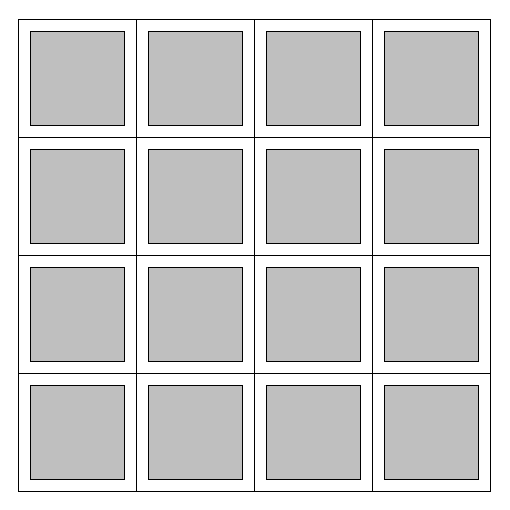
\includegraphics[width=1.8in]{amr4-1.eps} \ \
            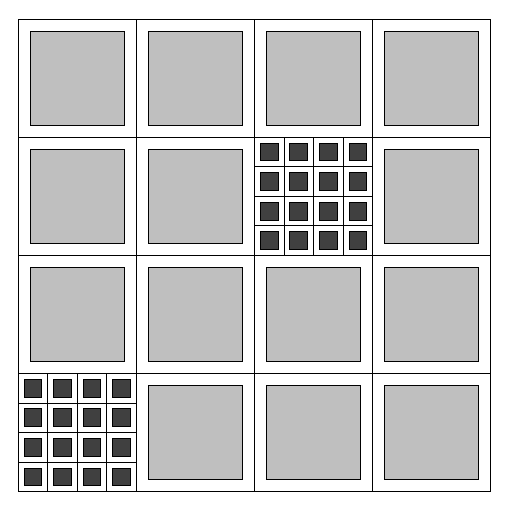
\includegraphics[width=1.8in]{amr4-2.eps} \ \
            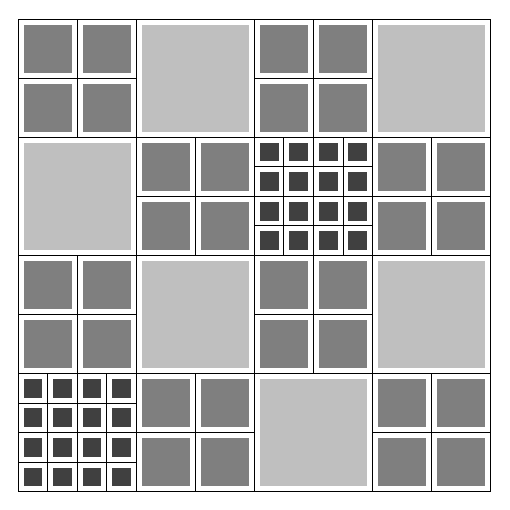
\includegraphics[width=1.8in]{amr4-3.eps}}

\centerline{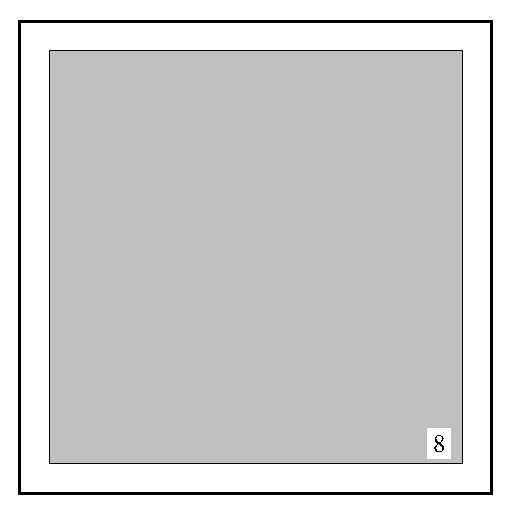
\includegraphics[width=1.8in]{amr2-1.eps} \ \
            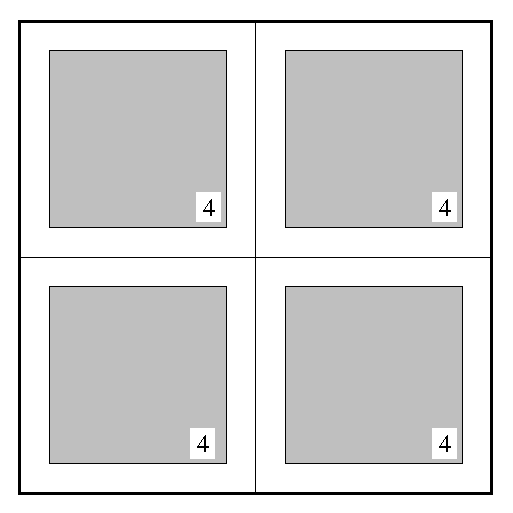
\includegraphics[width=1.8in]{amr2-2.eps} \ \
            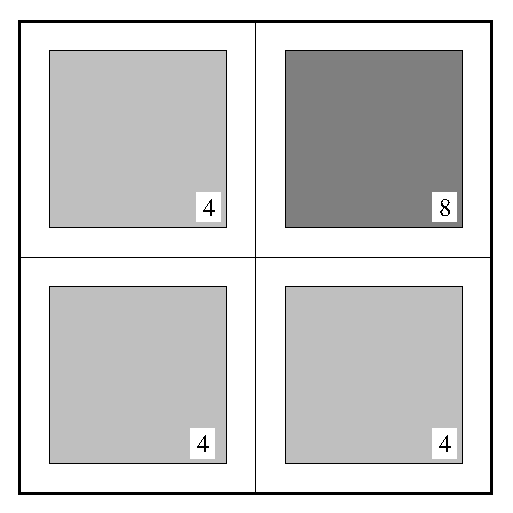
\includegraphics[width=1.8in]{amr2-3.eps}}
\ \\
\centerline{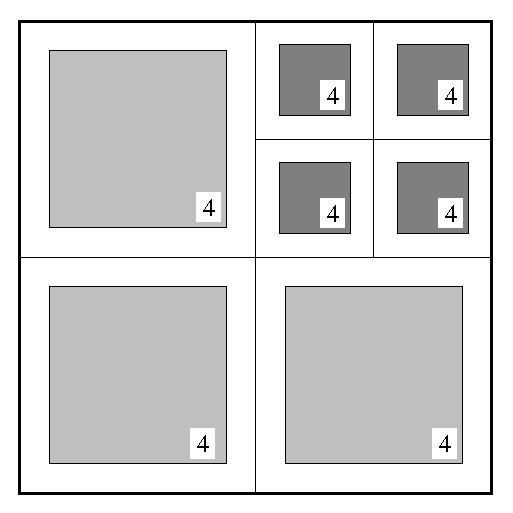
\includegraphics[width=1.8in]{amr2-4.eps} \ \
            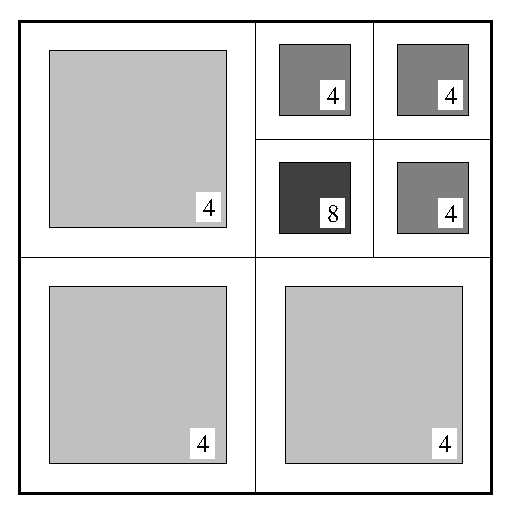
\includegraphics[width=1.8in]{amr2-5.eps} \ \
            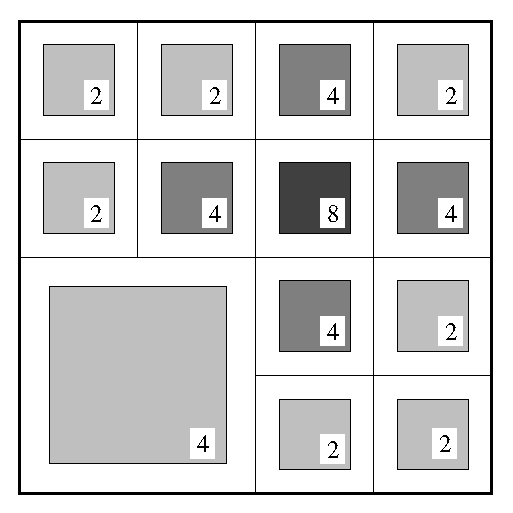
\includegraphics[width=1.8in]{amr2-7.eps}}
\ \\
\centerline{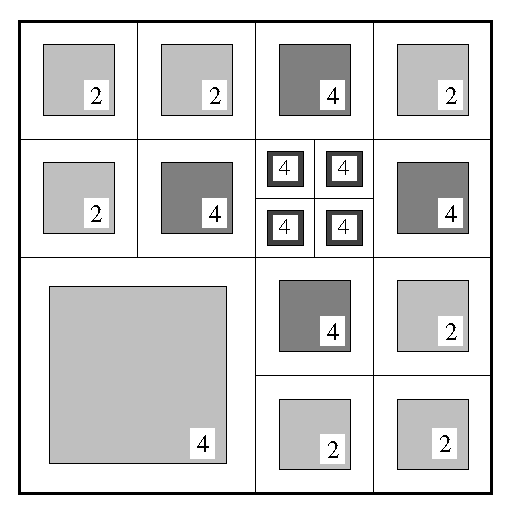
\includegraphics[width=1.8in]{amr2-8.eps} \ \
            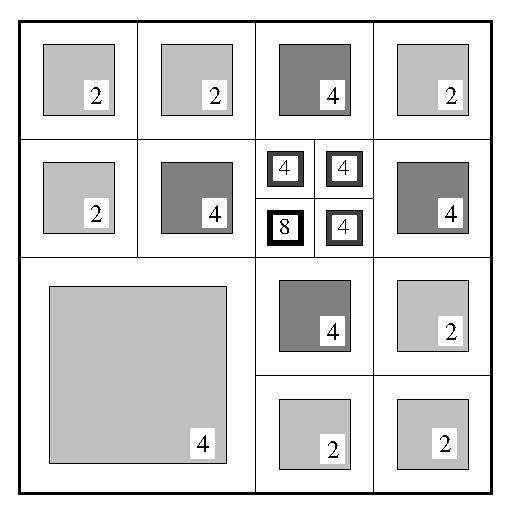
\includegraphics[width=1.8in]{amr2-9.eps} \ \
            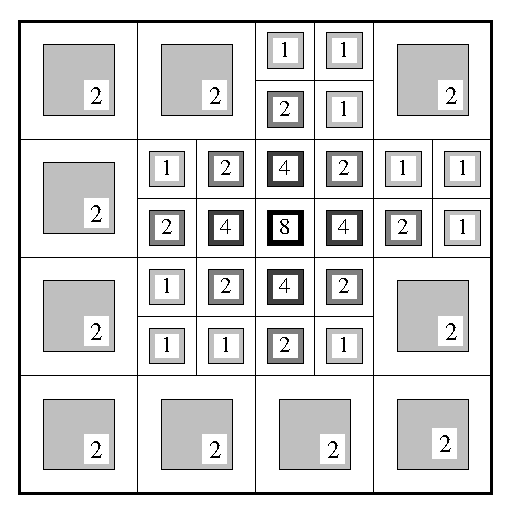
\includegraphics[width=1.8in]{amr2-11.eps}}

%-----------------------------------------------------------------------
\subsection{Use Cases}
%-----------------------------------------------------------------------
%-----------------------------------------------------------------------
\subsection{Parameters}
%-----------------------------------------------------------------------

%=======================================================================
\section{Particles Component} \label{s:component-particles}
%=======================================================================

Specifies data structures and data structure parameters related
to distributed particles.  

\begin{itemize}
\item min\_group\_size
\item max\_group\_size
\end{itemize}

%-----------------------------------------------------------------------
\subsection{Use Cases}
%-----------------------------------------------------------------------
%-----------------------------------------------------------------------
\subsection{Parameters}
%-----------------------------------------------------------------------


%=======================================================================
\section{Parallel Component} \label{s:component-parallel}
%=======================================================================

Hardware platform parallelism will be considered to be multilevel,
including nodes, processors, and cores.  Computational tasks will be
flexibly organized into hierarchical levels to aid mapping to multiple
hardware parallelization levels, including grid patches, grid patch
subblocks, and multiple simulations.  Task sizes in different levels
will allow flexibility to help optimize granularity for the different
given parallelization level components.

Flexible parallelism paradigms: map parallelism to tasks

Automatic code generation (or other) of parallel tasks to implement
parallelism and optimize performance

Specify parallelism type and parameters.  For example, non-blocking
MPI, MPI-2, hybrid MPI/UPC, performance-related parameters such as
buffer size, etc.

Specifiy parallelism and parameters

Specifiy method for controling parallelism

   parallelization method (MPI buffered/blocking, MPI2 Get)

\begin{itemize}
\item MPI (send/recv and type, one-sided and type, what level)
\item OpenMP (num threads, what level)
\item UPC (num threads, what level)
\item pthreads (num threads, what level)
\item cooperative parallelism
\item levels for each if multiple
\end{itemize}

%-----------------------------------------------------------------------
\subsection{Use Cases}
%-----------------------------------------------------------------------
%-----------------------------------------------------------------------
\subsection{Parameters}
%-----------------------------------------------------------------------

%=======================================================================
\subsection{MPI Send/Recv}

%=======================================================================
\subsection{MPI2 Get}

%=======================================================================
\subsection{OpenMP}

%=======================================================================
\subsection{Collaberative parallelism}

%=======================================================================
\subsection{Pipelining}




%=======================================================================
\section{Performance parameters} \label{s:performance}
%=======================================================================

Performance monitoring and optimization(?) parameters

%-----------------------------------------------------------------------
\subsection{Use Cases}
%-----------------------------------------------------------------------
%-----------------------------------------------------------------------
\subsection{Parameters}
%-----------------------------------------------------------------------

%=======================================================================
\section{Monitor parameters} \label{s:monitor}
%=======================================================================

High-level monitoring of the run at a summary level, such as current
timestep, problem time, wall time, cpu time, etc.

%-----------------------------------------------------------------------
\subsection{Use Cases}
%-----------------------------------------------------------------------
\begin{verbatim}
   monitor {
     type   = html
     amount = verbose
   }
\end{verbatim}
%-----------------------------------------------------------------------
\subsection{Parameters}
%-----------------------------------------------------------------------

%=======================================================================
\section{Output parameters} \label{s:output}
%=======================================================================

Output parameters.

%-----------------------------------------------------------------------
\subsection{Use Cases}
%-----------------------------------------------------------------------

\begin{verbatim}
output { 
   name = "data"
   format = hdf5
   type   = [data, input]
   fields = ["density", "velocity", "temperature"]
   file = ["data-%6s" cycle_number]
   cycle = 0:10:90
   cycle = 100:100:900
   cycle = 1000
}
\end{verbatim}

\begin{verbatim}
output { 
   name      = "restart"
   format    = hdf5
   type      = [data, input]
   fields    = all
   file      = ["restart-%6s" cycle_number]
   time_cpu  = 0.5 # CPU hours
   overwrite = true
   copies    = 2
}
\end{verbatim}

\begin{verbatim}
output { 
   name      = "movie"
   file      = ["movie-%6s" cycle_number]
   time      = :10:
   extract   = x == 12
}
\end{verbatim}


%-----------------------------------------------------------------------
\subsection{Parameters}
%-----------------------------------------------------------------------



%=======================================================================
\section{Recover Component} \label{s:component-recover}
%=======================================================================

Fault tolerance and adaptivity parameters

\begin{itemize}
\item fault tolerance methodology
\item adaptivity
\end{itemize}

%-----------------------------------------------------------------------
\subsection{Use Cases}
%-----------------------------------------------------------------------
%-----------------------------------------------------------------------
\subsection{Parameters}
%-----------------------------------------------------------------------



%======================================================================@



%======================================================================@
\chapter{Classes} \label{c:classes}
%======================================================================@


%======================================================================@
\chapter{Problem Classes} \label{s:problem-classes}
%======================================================================@

%=======================================================================
\section{\code{Simulation} class}
%=======================================================================

The \code{Simulation} class is used to define a simulation.  
\begin{itemize}
\item \code{Problem}
\end{itemize}

\subsection{Attributes.}

\subsection{Operations}

%=======================================================================
\section{\code{Parameters} class}
%=======================================================================

The \code{Parameters} class read in a parameter file or files, and
provide the application access to parameter values.


\subsection{Attributes}

\subsection{Operations}

%=======================================================================
\section{\code{Physics} class}
%=======================================================================


\subsection{Attributes}

\subsection{Operations}

%=======================================================================
\section{\code{Domain} class}
%=======================================================================

The \code{Domain} class defines the problem domain


\subsection{Attributes}

\subsection{Operations}

%=======================================================================
\section{\code{BC} class}
%=======================================================================

The \code{BC} class defines boundary conditions on a \code{Domain}.



\subsection{Attributes}

\subsection{Operations}

%=======================================================================
\section{\code{IC} class}
%=======================================================================

The \code{IC} class defines initial conditions for a set of
\code{Field}s in a \code{Domain}.


\subsection{Attributes}

\subsection{Operations}

%=======================================================================
\section{\code{Problem} class}
%=======================================================================

The \code{Problem} class defines the problem to be solved, including
the domain, boundary conditions, and initial field values.


\subsection{Attributes}

\subsection{Operations}

%=======================================================================
\section{\code{Field} class} \label{ss:field}
%=======================================================================

A \code{Field} represents a discrete multiresolution scalar or vector
field.  A \code{Field} is associated with a \code{Hierarchy}, and is
composed of \code{Array}'s defined on a subset of \code{Grid}s in the
\code{Hierarchy}.

\subsection{Attributes}

\subsection{Operations}

%=======================================================================
\section{\code{Units} class}
%=======================================================================

A \code{Units} class represents the physical units for the data in a
\code{Field}.

\subsection{Attributes}

\subsection{Operations}

\newpage

%======================================================================@
\chapter{Data Classes} \label{s:data-classes}
%======================================================================@

\centerline{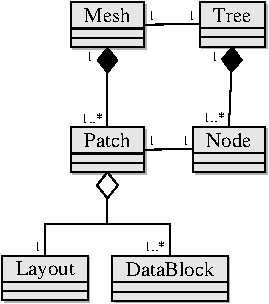
\includegraphics{uml/amr.1}}

%=======================================================================
\section{\code{Hierarchy} class}
%=======================================================================

A \code{Hierarchy} class represents a distributed structured AMR grid
hierarchy.  A \code{Hierarchy} can be considered to be an aggregate of
\code{Level}s, each of which in turn is an aggregate of individual
\code{Patch}es.  A patch is composed of a \code{Box}, which defines
the position and size in space, and some number of \code{Array}s, which
are used to store \code{Field} data (see \S\ref{ss:field}).



\subsection{Attributes}

\subsection{Operations}

%=======================================================================
\section{\code{Level} class}
%=======================================================================

A \code{Level} class represents a level in a distributed structured
AMR grid hierarchy (\code{Hierarchy}, where a level is defined as all
grid patches (\code{Grid}s) that have the same resolution.  A
\code{Level} is usually contained in a \code{Hierarchy}.

% The AMR hierarchy is represented using the trio of classes
% \code{Hierarchy}, \code{Level}, and \code{Grid}.
%   A \code{Grid} is a
% box in space, and is decomposed into \code{GridLocal} and
% \code{GridRemote} classes (see \S\ref{sss:class-grid}).  Each
% \code{GridLocal} object has some number of \code{Field} objects
% associated with them (see \S\ref{sss:class-field}), though the
% \code{GridLocal} objects themselves do not store field data
% themselves.  A \code{Level} class is also either a ``structured''
% \code{LevelStruct} or an ``unstructured'' \code{LevelUnstruct}.
% Structured levels are composed of a regular array of \code{Grid}s, and
% is typically used for unigrid calculations or the root level of an AMR
% calculation.  Unstructured levels are typically used for non-root
% levels of an AMR calulation.

\subsection{Attributes}

\subsection{Operations}

%=======================================================================
\section{\code{Patch} class}
%=======================================================================

A \code{Patch} class represents a grid patch in a distributed structured
AMR grid hierarchy (\code{Hierarchy}).  A \code{Patch} is defined by a
\code{Box}, and a set of \code{Array}s defined on the \code{Patch}.  Each
\code{Patch} is contained within a \code{Level}, and may be distributed
according to a \code{Parallel} object \S\ref{ss:parallel}.

\subsection{Attributes}

\subsection{Operations}

%=======================================================================
\section{\code{Box} class}
%=======================================================================

The \code{Box} class is for representing a box, and provides KeLP-like functionality.
Boxes are determined by two points, which may be of any parameterized type
(e.g.~\code{int} or \code{double}, etc.).


\subsection{Attributes}

\subsection{Operations}

%=======================================================================
\section{\code{Array} class}
%=======================================================================

The \code{Array} class encapsulates Fortran-style arrays with
convenient operations.  \code{Array}s may have optional support for
storing blocked or chunked arrays, include array padding, or store
interleaved arrays.  Arrays may be parallelized according to an
associated (static?) \code{Parallel} object (\S\ref{ss:parallel}).

% \centerline{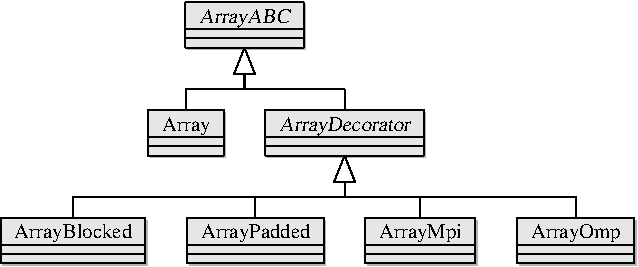
\includegraphics{uml/arrays.1}}

% \centerline{\includegraphics{uml/arrayabc.1}}

\centerline{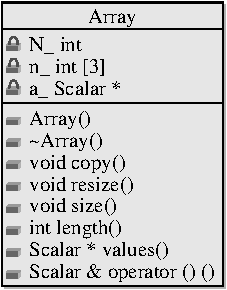
\includegraphics{uml/array.1}}

\subsubsection{Array shape}

\subsubsection{Array blocking}

\subsubsection{Array padding}

\subsubsection{Array interleaving}


\subsection{Attributes}

\begin{tabbing}
xx\=xx\=xxxxxxxxxxxxxxxxxxxxxxxxxxxxxxxxxxx\= \kill
\> \todo \>  \textit{Length of array} \\
\>       \> \code{N\_: int }      \\ \\
\> \todo \>  \textit {Shape of array, right-padded with 1's} \\
\>       \> \code{n\_: int [3] }  \\ \\
\> \todo \>  \textit {Array values stored in column-major ordering}\\
\>       \> \code{a\_: Scalar * }
\end{tabbing}

\subsection{Operations}

\begin{tabbing}
xx\=xx\=xxxxxxxxxxxxxxxxxxxxxxxxxxxxxxxxxxx\= \kill
\> \todo \> \textit{Create a new uninitialized Array object} \\
\>       \> \code{Array()} \\ \\
\> \todo \> \textit{Create a new initialized Array object} \\
\>       \> \code{Array(int n0, int n1=1, int n2=1, int n3=1)} \\ \\
\> \todo \> \textit{Deallocate the array} \\
\>       \> \code{\~{\ }Array()}  \\ \\
\> \todo \> \textit{Copy an array into this one, deallocating any existing data} \\
\>       \> \code{void copy (const Array \&)}  \\ \\
\> \todo \> \textit{Resize the array, deallocating any existing data} \\
\>       \> \code{void resize (int n0, int n1=1, int n2=1, int n3=1)}   \\ \\
\> \todo \> \textit{Return the size of the array} \\
\>       \> \code{void size (int *n0, int *n1=0, int *n2=0, int *n3=0) const}  \\ \\
\> \todo \> \textit{Return the total length of the array} \\
\>       \> \code{int length () const}  \\ \\
\> \todo \> \textit{Return a pointer to the array values} \\
\>       \> \code{Scalar * values () const}  \\ \\
\> \todo \> \textit{Return the given array element} \\
\>       \> \code{Scalar \& operator () (int i0, int i1=0, int i2=0, int i3=0)}
\end{tabbing}



   \devel{User interface: output.}
   
   \devel{User interface: portal.}
   The application will include a means for external applications to
   ``attach'' to the application (in a read-only sense) to access
   the data as it is being computed.  The purpose is to enable 
   external analysis and visualization tools to input data from the
   running application, providing the user with immediate
   feedback on the state and progress of the running simulation(s).

%  I/O

   \devel{Output.}
   Several options for how data fields and particles are read and
   stored to disk will be implemented, to improve flexibility and
   allow optimization of I/O for a given problem on a given parallel
   platform.  Parallel HDF5 will be used to optimize efficiency and
   portability.  Multiple data layouts within and between files will
   be implemented to allow optimization of I/O to a particular problem
   and file system.

%  I/O dumps, inline analysis, visualization

   Support will be available for writing the whole or part of some or
   all data fields and particles at specified times.  I/O dumps will
   include targeted support for both check-pointing (for automatic use
   by the software error recovery) and data dumps (for subsequent user
   use).  
   
%  Error recovery

   Support will be included for error prevention, identification and
   recovery.  This will include fault-tolerance methods to handle
   possible hardware faults, and self-monitoring of fields, particles,
   and other variables against physics quantity invariants
   (e.g.~positive densities, mass conservation, etc.) to identify
   potential problems as soon after they occur as possible, so that
   the user or application can halt the simulation, or restart from
   an earlier snapshot using modified parameters for physics or
   methods.

% Self-tuning

   Support will be included for tuning of various components to the
   running application and hardware platform.  Tuning will be either
   self-tuning by the running application as it monitors its
   performance, or by the user monitoring the performance of a running
   simulation.  Adaptivity will be available for physics, physics
   methods, resolution ranges, AMR data-structures and algorithms,
   field and particles data-structures, and parallelism.

\begin{itemize}
\item Extreme scalability
\item Extreme efficiency
\item Easy for user to compile and run
\item Easy to developer to modify and maintain
\item Powerful problem definition
\item Flexibile algorithms and parallel datastructures
\item Rigorous testing of accuracy, performance and scalability
\end{itemize}

%=======================================================================
\section{Control parameters} \label{s:control}
%=======================================================================

Given Physics, Algorithms, and Data structures, specify the top-level
sequencing and properties of the simulation.  For example, ordering of
physics modules, whether to do hierarchical time-stepping, up to what
level, whether to sub-cycle some physics, etc. [Is this a useful
category?]  Also include things like floors and limits(?), and IO
dumps

Global simulation control.

Output types and parameters

\begin{itemize}
\item checkpoint (dump all)
\item output (specific fields)
\item movies (type and rate)
\item analysis (type of analysis, rate)
\item level of output (files for timestep, time, etc.)
\end{itemize}

%-----------------------------------------------------------------------
\subsection{Use Cases}
%-----------------------------------------------------------------------
%-----------------------------------------------------------------------
\subsection{Parameters}
%-----------------------------------------------------------------------

%=======================================================================
\section{Physics parameters} \label{s:physics}
%=======================================================================

Specify physics modules and physics parameters, including
hydrodynamics, self-gravity, gravitational constant, imposed gravity,
chemistry, cosmological expansion, star formation, etc.  Physics is in
the problem domain.

Specify physics components

\begin{itemize}
\item hydrodynamics
\item  cosmological expansion
\item self-gravity
\end{itemize}

%-----------------------------------------------------------------------
\subsection{Use Cases}
%-----------------------------------------------------------------------
%-----------------------------------------------------------------------
\subsection{Parameters}
%-----------------------------------------------------------------------

%=======================================================================
\section{Units parameters} \label{s:units}
%=======================================================================

 Specify units and optional scalings for individual
 fields.  [Merge units with Control?] [Merge scaling with Fields?] 
 [Dynamic scaling, e.g.~to keep average of all fields near one.]

%-----------------------------------------------------------------------
\subsection{Use Cases}
%-----------------------------------------------------------------------
%-----------------------------------------------------------------------
\subsection{Parameters}
%-----------------------------------------------------------------------

%=======================================================================
\section{Problem parameters} \label{s:problem}
%=======================================================================

Problem parameters include initial conditions and boundary conditions.

Different types of boundary conditions are supported, including
periodic, in- and out-flow, specified, and dynamic.  Different
boundary conditions can be specified for the entire domain, on
separate faces, on subregions of faces, or on specific zones.
Different boundary conditions can be specified for different fields.
%-----------------------------------------------------------------------
\subsection{Use Cases}
%-----------------------------------------------------------------------

\begin{verbatim}
   problem {
      boundary {
         x:lower = reflecting
         x:upper = { type = reflecting }
         y       = { type = periodic }
         z       = { type = inflow,  value = 1.0 }
         z       = { outflow, 1.0 }
      }
   }
\end{verbatim}

\begin{verbatim}
   XM = boundary { x = domain:lower[0] }
   XP = boundary { x = domain:upper[0] }
   YM = boundary { y = domain:lower[1] }
   YP = boundary { y = domain:upper[1] }
   ZM = boundary { z = domain:lower[2] }
   ZP = boundary { z = domain:upper[2] }
   field {
      name = "density"
      value(XM) = 0
      value(XP) = 0
      value(YM) = value (YP)
      value(ZM) = +t
      value(ZM) = -t
   }
\end{verbatim}

%-----------------------------------------------------------------------
\subsection{Parameters}
%-----------------------------------------------------------------------

%=======================================================================
\section{Domain parameters} \label{s:domain}
%=======================================================================

The \code{domain} function is used to specify properties of the
domain.  Domains are boxes aligned with the axes of the computational
coordinate system, and are uniquely determined by the spacial
dimension, and the lowest and highest points in the domain.

%-----------------------------------------------------------------------
\subsection{Use Cases}
%-----------------------------------------------------------------------

\begin{verbatim}
   domain { 
      dimension = 3
      lower     = <-3e9,-3e9,-3e9>
      upper     = <3e9,3e9,3e9>
   }
\end{verbatim}

\begin{verbatim}
   domain { 3, <-3e9,-3e9,-3e9>, <3e9,3e9,3e9> }  // Implicit ordering
\end{verbatim}

\begin{verbatim}
   domain { 
      dimension = 3
      upper     = 3e9        // expand scalar to vector
      lower     = -upper     // parameters can be accessed as values
   }
\end{verbatim}

Include errors.

%-----------------------------------------------------------------------
\subsection{Parameters}
%-----------------------------------------------------------------------

 \todo\ \textit{Decide: allow defaults?  allow optional parameters?  Special
 \code{OPT\_} prefix for optional parameters?  Write out explicit copy
 of input file?}

The \code{domain} function has three parameters

\begin{tabular}{lll} \\
Name & Type & Restrictions \\ \hline
\code{dimension} & Scalar & $1-3$ \\
\code{lower}     & Vector & length = \code{dimension} \\
\code{upper}     & Vector & length = \code{dimension}, \code{upper} $>$ \code{lower}
\end{tabular}

Lower and upper points are given in units given by \code{units},
described in \S\ref{s:units}.

%-----------------------------------------------------------------------
\subsection{Restrictions}
%-----------------------------------------------------------------------

\begin{enumerate}
\item The dimension must be 1, 2, or 3.
\item The number of coordinates in both lower and upper points must equal the dimension.
\item Each coordinate of the lower point must be strictly greater than the corresponding coordinate of the upper point.
\end{enumerate}


%=======================================================================
\section{Region parameters} \label{s:region}
%=======================================================================

Specify partitions of the domain into regions.  Each region contains
different materials with different properties.  Example partitions may
be half-planes, spheres, boxes, or specified using a file containing a
zone bit mask.  Default is region 0, first region is region 1, etc.
Use solid modeling representations?

%-----------------------------------------------------------------------
\subsection{Use Cases}
%-----------------------------------------------------------------------

\begin{verbatim}
   region {
      x + y + z < 0.5
   }
\end{verbatim}

\begin{verbatim}
   BOX = region {
      (x > 0) &&
      (x < 1) &&
      (y > 0) && (y < 1) &&
      (z > 0) && (z < 1)
   }
\end{verbatim}

\begin{verbatim}
   region {
      union {
         region {BOX, translate = 0.0*x, scale = 0.1}
         region {BOX, translate = 0.1*x, scale = <0.1,0.1,0.1>}
         region {BOX, translate = 0.2*x, scale = 0.1}
      }
   }
\end{verbatim}

\begin{verbatim}
   region {
      x = domain:lower[0]
   }
\end{verbatim}

\begin{verbatim}
   region {
      x*x + y*y + z*z < 1
   }
\end{verbatim}

\begin{verbatim}
   region {
      bitmask = "filename.hdf5"
   }
\end{verbatim}


%-----------------------------------------------------------------------
\subsection{Parameters}
%-----------------------------------------------------------------------

%=======================================================================
\section{Field parameters} \label{s:field}
%=======================================================================

Scalar and vector fields for each material, such as
 density, energy, velocity, etc.  [Merge with Materials?]  Specify
 values, or input from files.

%-----------------------------------------------------------------------
\subsection{Use Cases}
%-----------------------------------------------------------------------
\begin{verbatim}
   field {
      name     = "density"
      name     = "rho"
      type     = scalar
      location = center
   }
   field {
      name     = "velocity"
      name     = "u"
      type     = vector
      location = center
   }
   field {
      name     = "temperature"
      name     = "T"
      type     = scalar
      location = center
   }
   field {
      name     = "B"
      type     = computed
      location = face
   }
\end{verbatim}
%-----------------------------------------------------------------------
\subsection{Parameters}
%-----------------------------------------------------------------------

%=======================================================================
\section{Matter parameters} \label{s:matter}
%=======================================================================

 Matter defines properties of matter, such as the matter type (baryonic
 or dark matter), and gas constants.

%-----------------------------------------------------------------------
\subsection{Use Cases}
%-----------------------------------------------------------------------

\begin{verbatim}
   Matter {
      type = dark
   }
\end{verbatim}

\begin{verbatim}
   Matter {
      type  = gas_ideal
      gamma = 1.4
      region { (x < 0) || (x > 1) }
   }
\end{verbatim}
%-----------------------------------------------------------------------
\subsection{Parameters}
%-----------------------------------------------------------------------

%=======================================================================
\section{Method parameters} \label{s:method}
%=======================================================================

 Specify the algorithms and algorithm parameters
 to use for each physics component.  Each physics component has a
 default; some components may have only one available
 (e.g.~cosmological expansion).  Algorithms is in the solution domain.

\begin{itemize}
\item PPM hydro (dual-energy, etc.)
\item gravity solver (FAC, smoother, levels, etc.)
\end{itemize}

%-----------------------------------------------------------------------
\subsection{Use Cases}
%-----------------------------------------------------------------------
%-----------------------------------------------------------------------
\subsection{Parameters}
%-----------------------------------------------------------------------

%=======================================================================
\section{AMR data structure parameters} \label{s:amr}
%=======================================================================

Specify data structures and data structure parameters for distributed
AMR hierarchies, such as number of mesh levels, grid patch properties,
rebuild algorithm, dynamic load balancing, refinement criteria, etc.

\begin{itemize}
\item hierarchy
\begin{item}
\item min\_levels 
\item max\_levels 
\end{item}
\item level
\item grid
\begin{itemize}
\item min\_size
\item max\_size
\item max\_aspect
\item quantum
\end{itemize}
\end{itemize}

%-----------------------------------------------------------------------
\subsection{Use Cases}
%-----------------------------------------------------------------------
%-----------------------------------------------------------------------
\subsection{Parameters}
%-----------------------------------------------------------------------

%=======================================================================
\section{Particle parameters} \label{s:data}
%=======================================================================

Specifies data structures and data structure parameters related
to distributed particles.  

\begin{itemize}
\item min\_group\_size
\item max\_group\_size
\end{itemize}

%-----------------------------------------------------------------------
\subsection{Use Cases}
%-----------------------------------------------------------------------
%-----------------------------------------------------------------------
\subsection{Parameters}
%-----------------------------------------------------------------------

%=======================================================================
\section{Parallel parameters} \label{s:parallel}
%=======================================================================

Specify parallelism type and parameters.  For example, non-blocking
MPI, MPI-2, hybrid MPI/UPC, performance-related parameters such as
buffer size, etc.

Specifiy parallelism and parameters

\begin{itemize}
\item MPI (send/recv and type, one-sided and type, what level)
\item OpenMP (num threads, what level)
\item UPC (num threads, what level)
\item pthreads (num threads, what level)
\item cooperative parallelism
\item levels for each if multiple
\end{itemize}

%-----------------------------------------------------------------------
\subsection{Use Cases}
%-----------------------------------------------------------------------
%-----------------------------------------------------------------------
\subsection{Parameters}
%-----------------------------------------------------------------------
%=======================================================================
\section{Performance parameters} \label{s:performance}
%=======================================================================

Performance monitoring and optimization(?) parameters

%-----------------------------------------------------------------------
\subsection{Use Cases}
%-----------------------------------------------------------------------
%-----------------------------------------------------------------------
\subsection{Parameters}
%-----------------------------------------------------------------------

%=======================================================================
\section{Monitor parameters} \label{s:monitor}
%=======================================================================

High-level monitoring of the run at a summary level, such as current
timestep, problem time, wall time, cpu time, etc.

%-----------------------------------------------------------------------
\subsection{Use Cases}
%-----------------------------------------------------------------------
\begin{verbatim}
   monitor {
     type   = html
     amount = verbose
   }
\end{verbatim}
%-----------------------------------------------------------------------
\subsection{Parameters}
%-----------------------------------------------------------------------

%=======================================================================
\section{Output parameters} \label{s:output}
%=======================================================================

Output parameters.

%-----------------------------------------------------------------------
\subsection{Use Cases}
%-----------------------------------------------------------------------

\begin{verbatim}
output { 
   name = "data"
   format = hdf5
   type   = [data, input]
   fields = ["density", "velocity", "temperature"]
   file = ["data-%6s" cycle_number]
   cycle = 0:10:90
   cycle = 100:100:900
   cycle = 1000
}
\end{verbatim}

\begin{verbatim}
output { 
   name      = "restart"
   format    = hdf5
   type      = [data, input]
   fields    = all
   file      = ["restart-%6s" cycle_number]
   time_cpu  = 0.5 # CPU hours
   overwrite = true
   copies    = 2
}
\end{verbatim}

\begin{verbatim}
output { 
   name      = "movie"
   file      = ["movie-%6s" cycle_number]
   time      = :10:
   extract   = x == 12
}
\end{verbatim}


%-----------------------------------------------------------------------
\subsection{Parameters}
%-----------------------------------------------------------------------

%=======================================================================
\section{Recovery parameters} \label{s:recovery}
%=======================================================================

Fault tolerance and adaptivity parameters.

\begin{itemize}
\item Power outage
\item Network connectivity dropouts
\item Corrupt RAM
\item Crashed hard drive
\item Moth in relay switch
\item Crashed node
\end{itemize}

\begin{itemize}
\item fault tolerance methodology
\item adaptivity
\end{itemize}

%-----------------------------------------------------------------------
\subsection{Use Cases}
%-----------------------------------------------------------------------
%-----------------------------------------------------------------------
\subsection{Parameters}
%-----------------------------------------------------------------------

%=======================================================================
\chapter{Outputs} \label{c:outputs}
%=======================================================================

%=======================================================================
\chapter{Functional Requirements}
%=======================================================================

%=======================================================================
\section{Control}
%=======================================================================

%=======================================================================
\section{Physics}
%=======================================================================

%=======================================================================
\subsection{Hydrodynamics}

%=======================================================================
\subsection{Self-gravity}

%=======================================================================
\subsection{MHD}

%=======================================================================
\subsection{RT}

%=======================================================================
\section{Data-Structures}
%=======================================================================

%=======================================================================
\subsection{Arrays}

%=======================================================================
\subsection{Fields}

%=======================================================================
\subsection{Particles}

%=======================================================================
\subsection{Structured Adaptive Mesh Hierarchies}

%=======================================================================
\subsection{Octree}

%=======================================================================
\section{Parallelism}
%=======================================================================

Hardware platform parallelism will be considered to be multilevel,
including nodes, processors, and cores.  Computational tasks will be
flexibly organized into hierarchical levels to aid mapping to multiple
hardware parallelization levels, including grid patches, grid patch
subblocks, and multiple simulations.  Task sizes in different levels
will allow flexibility to help optimize granularity for the different
given parallelization level components.

Flexible parallelism paradigms: map parallelism to tasks

Automatic code generation (or other) of parallel tasks to implement
parallelism and optimize performance

%=======================================================================
\subsection{MPI Send/Recv}

%=======================================================================
\subsection{MPI2 Get}

%=======================================================================
\subsection{OpenMP}

%=======================================================================
\subsection{Collaberative parallelism}

%=======================================================================
\subsection{Pipelining}

\appendix
\newcommand{\parametersize}{\scriptsize}

%=======================================================================
\chapter{\enzo\ parameters list}
%=======================================================================

\small
\begin{tabular}{lll}
\todo\ \code{AdjustUVBackground} &
\todo\ \code{BaryonSelfGravityApproximation} &
\todo\ \code{BoundaryConditionName} \\
\todo\ \code{CellFlaggingMethod} &
\todo\ \code{ComovingCoordinates} &
\todo\ \code{ComputePotential} \\
\todo\ \code{ConservativeInterpolation} &
\todo\ \code{CoolDataParamfile} &
\todo\ \code{CourantSafetyNumber} \\
\todo\ \code{CubeDumpEnabled} &
\todo\ \code{CubeDump} &
\todo\ \code{CycleLastDataDump} \\
\todo\ \code{CycleLastHistoryDump} &
\todo\ \code{CycleLastRestartDump} &
\todo\ \code{CycleSkipDataDump} \\
\todo\ \code{CycleSkipGlobalDataDump} &
\todo\ \code{CycleSkipHistoryDump} &
\todo\ \code{CycleSkipRestartDump} \\
\todo\ \code{DataDumpDir} &
\todo\ \code{DataDumpName} &
\todo\ \code{DataDumpNumber} \\
\todo\ \code{DataLabel} &
\todo\ \code{DataUnits} &
\todo\ \code{DomainLeftEdge} \\
\todo\ \code{DomainRightEdge} &
\todo\ \code{dtDataDump} &
\todo\ \code{dtHistoryDump} \\
\todo\ \code{dtMovieDump} &
\todo\ \code{dtRestartDump} &
\todo\ \code{dtTracerParticleDump} \\
\todo\ \code{DualEnergyFormalismEta1} &
\todo\ \code{DualEnergyFormalismEta2} &
\todo\ \code{DualEnergyFormalism} \\
\todo\ \code{ExternalBoundaryIO} &
\todo\ \code{ExternalBoundaryTypeIO} &
\todo\ \code{ExternalBoundaryValueIO} \\
\todo\ \code{ExtractFieldsOnly} &
\todo\ \code{FluxCorrection} &
\todo\ \code{GadgetEquilibriumCooling} \\
\todo\ \code{Gamma} &
\todo\ \code{GlobalDir} &
\todo\ \code{GravitationalConstant} \\
\todo\ \code{GravityBoundaryFaces} &
\todo\ \code{GravityBoundaryName} &
\todo\ \code{GravityBoundaryRestart} \\
\todo\ \code{GravityResolution} &
\todo\ \code{GreensFunctionMaxNumber} &
\todo\ \code{GreensFunctionMaxSize} \\
\todo\ \code{GridVelocity} &
\todo\ \code{HistoryDumpDir} &
\todo\ \code{HistoryDumpName} \\
\todo\ \code{HistoryDumpNumber} &
\todo\ \code{huge\_number} &
\todo\ \code{HydroMethod} \\
\todo\ \code{InitialCPUTime} &
\todo\ \code{InitialCycleNumber} &
\todo\ \code{Initialdt} \\
\todo\ \code{InitialTime} &
\todo\ \code{InterpolationMethod} &
\todo\ \code{LeftFaceBoundaryCondition} \\
\todo\ \code{LocalDir} &
\todo\ \code{MaximumGravityRefinementLevel} &
\todo\ \code{MaximumParticleRefinementLevel} \\
\todo\ \code{MaximumRefinementLevel} &
\todo\ \code{MaximumSubgridSize} &
\todo\ \code{MinimumEfficiency} \\
\todo\ \code{MinimumEnergyRatioForRefinement} &
\todo\ \code{MinimumMassForRefinement} &
\todo\ \code{MinimumMassForRefinementLevelExponent} \\
\todo\ \code{MinimumOverDensityForRefinement} &
\todo\ \code{MinimumPressureJumpForRefinement} &
\todo\ \code{MinimumPressureSupportParameter} \\
\todo\ \code{MinimumShearForRefinement} &
\todo\ \code{MinimumSlopeForRefinement} &
\todo\ \code{MinimumSubgridEdge} \\
\todo\ \code{MovieDataField} &
\todo\ \code{MovieDumpDir} &
\todo\ \code{MovieDumpName} \\
\todo\ \code{MovieDumpNumber} &
\todo\ \code{MovieRegionLeftEdge} &
\todo\ \code{MovieRegionRightEdge} \\
\todo\ \code{MovieSkipTimestep} &
\todo\ \code{MultiMetals} &
\todo\ \code{MultiSpecies} \\
\todo\ \code{MustRefineParticlesRefineToLevel} &
\todo\ \code{NewMovieDumpNumber} &
\todo\ \code{NewMovieLeftEdge} \\
\todo\ \code{NewMovieName} &
\todo\ \code{NewMovieParticleOn} &
\todo\ \code{NewMovieRightEdge} \\
\todo\ \code{NumberOfBufferZones} &
\todo\ \code{NumberOfParticleAttributes} &
\todo\ \code{NumberOfParticles} \\
\todo\ \code{OutputFirstTimeAtLevel} &
\todo\ \code{ParallelParticleIO} &
\todo\ \code{ParallelRootGridIO} \\
\todo\ \code{ParticleBoundaryType} &
\todo\ \code{ParticleCourantSafetyNumber} &
\todo\ \code{ParticleTypeInFile} \\
\todo\ \code{ParticleTypeInFile} &
\todo\ \code{PartitionNestedGrids} &
\todo\ \code{PointSourceGravityConstant} \\
\todo\ \code{PointSourceGravityCoreRadius} &
\todo\ \code{PointSourceGravity} &
\todo\ \code{PointSourceGravityPosition} \\
\todo\ \code{PPMDiffusionParameter} &
\todo\ \code{PPMFlatteningParameter} &
\todo\ \code{PPMSteepeningParameter} \\
\todo\ \code{PressureFree} &
\todo\ \code{ProblemType} &
\todo\ \code{RadHydroParamfile} \\
\todo\ \code{RadiationFieldLevelRecompute} &
\todo\ \code{RadiationFieldType} &
\todo\ \code{RadiationHydrodynamics} \\
\todo\ \code{RadiationSpectrumNormalization} &
\todo\ \code{RadiationSpectrumSlope} &
\todo\ \code{RadiativeCooling} \\
\todo\ \code{RandomForcingEdot} &
\todo\ \code{RandomForcing} &
\todo\ \code{RandomForcingMachNumber} \\
\todo\ \code{RedshiftDumpDir} &
\todo\ \code{RedshiftDumpName} &
\todo\ \code{RefineBy} \\
\todo\ \code{RefineByJeansLengthSafetyFactor} &
\todo\ \code{RefineRegionLeftEdge} &
\todo\ \code{RefineRegionRightEdge} \\
\todo\ \code{RestartDumpDir} &
\todo\ \code{RestartDumpName} &
\todo\ \code{RestartDumpNumber} \\
\todo\ \code{RightFaceBoundaryCondition} &
\todo\ \code{S2ParticleSize} &
\todo\ \code{SelfGravity} \\
\todo\ \code{SetHeIIHeatingScale} &
\todo\ \code{SetUVBAmplitude} &
\todo\ \code{SRBprefix} \\
\todo\ \code{StarEnergyToQuasarUV} &
\todo\ \code{StarEnergyToStellarUV} &
\todo\ \code{StarEnergyToThermalFeedback} \\
\todo\ \code{StarMakerMassEfficiency} &
\todo\ \code{StarMakerMinimumDynamicalTime} &
\todo\ \code{StarMakerMinimumMass} \\
\todo\ \code{StarMakerOverDensityThreshold} &
\todo\ \code{StarMassEjectionFraction} &
\todo\ \code{StarMetalYield} \\
\todo\ \code{StarParticleCreation} &
\todo\ \code{StarParticleFeedback} &
\todo\ \code{StaticHierarchy}
\end{tabular}

\begin{tabular}{lll}
\todo\ \code{StaticRefineRegionLeftEdge} &
\todo\ \code{StaticRefineRegionLevel} &
\todo\ \code{StaticRefineRegionRightEdge} \\
\todo\ \code{StopCPUTime} &
\todo\ \code{StopCycle} &
\todo\ \code{StopFirstTimeAtLevel} \\
\todo\ \code{StopTime} &
\todo\ \code{TimeActionParameter} &
\todo\ \code{TimeActionParameter} \\
\todo\ \code{TimeActionRedshift} &
\todo\ \code{TimeActionRedshift} &
\todo\ \code{TimeActionTime} \\
\todo\ \code{TimeActionTime} &
\todo\ \code{TimeActionType} &
\todo\ \code{TimeLastDataDump} \\
\todo\ \code{TimeLastHistoryDump} &
\todo\ \code{TimeLastMovieDump} &
\todo\ \code{TimeLastRestartDump} \\
\todo\ \code{TimeLastTracerParticleDump} &
\todo\ \code{tiny\_number} &
\todo\ \code{TopGridDimensions} \\
\todo\ \code{TopGridGravityBoundary} &
\done\ \code{TopGridRank} &
\todo\ \code{TracerParticleDumpDir} \\
\todo\ \code{TracerParticleDumpName} &
\todo\ \code{TracerParticleDumpNumber} &
\todo\ \code{TracerParticleOn} \\
\todo\ \code{UniformGravityConstant} &
\todo\ \code{UniformGravityDirection} &
\todo\ \code{UniformGravity} \\
\todo\ \code{Unigrid} &
\todo\ \code{UseMinimumPressureSupport} &
\todo\ \code{VersionNumber} \\
\todo\ \code{WritePotential} &
\todo\ \code{ZEUSLinearArtificialViscosity} &
\todo\ \code{ZEUSQuadraticArtificialViscosity}
\end{tabular}

%=======================================================================
\chapter{\cello\ parameters list}
%=======================================================================

\small
\begin{tabular}{lll}
\todo\ \code{simulation:stop:time}  \\
\todo\ \code{simulation:stop:cycle} \\
\todo\ \code{simulation:stop:level} \\
\todo\ \code{simulation:stop:time:cpu} \\
\todo\ \code{simulation:stop:time:wall} \\
\todo\ \code{simulation:dimension} \\
\todo\ \code{simulation:type} \\
\todo\ \code{discretize:root:size} \\
\todo\ \code{domain:lower} \\
\todo\ \code{domain:upper} \\
\todo\ \code{BC:type:[x$|$y$|$z]\_[lower$|$upper]} \\
\todo\ \code{BC:value:[x$|$y$|$z]\_[lower$|$upper]} \\
\todo\ \code{IC:start:time} \\
\todo\ \code{IC:start:cycle} \\
\todo\ \code{output:time:period} \\
\todo\ \code{output:time:name} \\
\todo\ \code{output:time:value} \\
\todo\ \code{output:time:fields} \\
\todo\ \code{output:cycle:period} \\
\todo\ \code{output:cycle:name} \\
\todo\ \code{output:cycle:value} \\
\todo\ \code{output:cycle:fields} \\
\todo\ \code{output:type}\\
\todo\ \code{output:xray:lower} \\
\todo\ \code{output:xray:upper} \\
\todo\ \code{output:xray:range} \\
\todo\ \code{output:region}  \\
\todo\ \code{output:lower}  \\
\todo\ \code{output:upper}  \\
\todo\ \code{output:levels} \\
\todo\ \code{output:start:level} \\
\todo\ \code{monitor}\\
\todo\ \code{datastructure:type} \\
\todo\ \code{datastructure:type:samr:levels} \\
\todo\ \code{datastructure:type:samr:static} \\
\todo\ \code{datastructure:type:samr:dynamic} \\
\todo\ \code{refinement:factor} \\
\todo\ \code{refinement:criteria}
\todo\ \code{refinement:criteria:slope} \\
\todo\ \code{refinement:criteria:matter-baryon} \\
\todo\ \code{refinement:criteria:matter-dark} \\
\todo\ \code{refinement:criteria:shock} \\
\todo\ \code{refinement:criteria:Jeans} \\
\todo\ \code{refinement:criteria:cool} \\
\todo\ \code{refinement:region} \\
\todo\ \code{field:name} \\
\todo\ \code{field:type} \\
\todo\ \code{field:where} \\
\todo\ \code{method:hydro} \\
\todo\ \code{method:hydro:ppm} \\
\todo\ \code{method:hydro:ppm:dual-energy} \\
\todo\ \code{method:hydro:ppm:pressure-free} \\
\todo\ \code{method:hydro:ppm:flattening} \\
\todo\ \code{method:hydro:ppm:diffusion} \\
\todo\ \code{method:gravity} \\
\todo\ \code{method:flux-correct} \\
\todo\ \code{method:interpolate} \\
\todo\ \code{timestep:start:level} \\
\todo\ \code{timestep:cfl} \\
\todo\ \code{timestep:cfl:particles} \\
\todo\ \code{units:time} \\
\todo\ \code{units:distance} \\
\todo\ \code{cosmology:omega-lambda-now} \\
\todo\ \code{cosmology:hubble-lambda-now} \\
\todo\ \code{numerics:integer} \\
\todo\ \code{numerics:real} \\
\todo\ \code{particles:type} \\
\todo\ \code{particles:attribute-count} \\
\todo\ \code{particles:attribute-names} \\
\todo\ \code{parallel:grids} \\
\todo\ \code{parallel:subgrids} \\
\todo\ \code{physics:gravity:source} \\
\todo\ \code{physics:gravity} \\
\todo\ \code{physics:radiative-cooling} \\
\todo\ \code{physics:star-formation} \\
\todo\ \code{physics:radiation} \\
\todo\ \code{physics:magnetism} \\
\end{tabular}


\section{Types}

integer,real,string,vector,list,range,boolean

\section{Functions}

\code{abs()},
\code{min()},
\code{max()},
\code{sqrt()},
\code{exp()},
\code{avg()},
\code{log()}

\section{Variables and constants}

\code{x y z},
\code{t}

\code{PI}

\section{Operations}

\subsection{scalar operations}
$x + y$,
$x - y$,
$x * y$,
$x / y$

\subsection{logical operations}

$x < y$
$x <= y$
$x > y$
$x >= y$
$A \&\& B$
$A || B$
$A == B$
$A != B$

\subsection{region operations}

$R + S$
$R - S$
$-S$

\subsection{discrete field operations}

$E$, $I$, $D$, $_i$

\subsection{list operations}

* (cross-product)

\section{parameter restrictions}

\todo \textit{list constraints on parameters}

%=======================================================================
\chapter{\enzo\ versus \cello\ parameter files}
%=======================================================================

%-----------------------------------------------------------------------
\section{AdiabaticExpansion} \label{s:AdiabaticExpansion}
%-----------------------------------------------------------------------

%-----------------------------------------------------------------------
\subsection{\enzo}
%-----------------------------------------------------------------------

{\parametersize
\begin{tabbing}
xxxxxxx\=xxxxxxxxxxxxxxxxxxxxxxxxxxxxxxxxxxxxxxx\=\kill
\> AdiabaticExpansionInitialTemperature \> 1000  \\
\> AdiabaticExpansionInitialVelocity    \> 100   \\
\> ComovingCoordinates        \> 1        \\
\> CosmologyComovingBoxSize   \> 64.0     \\
\> CosmologyHubbleConstantNow \> 0.5 \\
\> CosmologyInitialRedshift   \> 20       \\
\> CosmologyMaxExpansionRate  \> 0.01     \\
\> CourantSafetyNumber    \> 0.5 \\
\> dtDataDump             \> 80.0 \\
\> DualEnergyFormalism    \> 1       \\
\> Gamma                  \> 1.6667 \\
\> GravitationalConstant      \> 1       \\
\> LeftFaceBoundaryCondition  \> 3        \\
\> PPMDiffusionParameter  \> 0        \\
\> ProblemType                \> 22       \\
\> RightFaceBoundaryCondition \> 3 \\
\> SelfGravity                \> 0        \\
\> StaticHierarchy           \> 1     \\
\> TopGridDimensions          \> 8 \\
\> TopGridGravityBoundary     \> 0        \\
\> TopGridRank                \> 1
\end{tabbing}}

%-----------------------------------------------------------------------
\subsection{\cello}
%-----------------------------------------------------------------------

%-----------------------------------------------------------------------
\section{AMRCosmologySimulation} \label{s:AMRCosmologySimulation}
%-----------------------------------------------------------------------

%-----------------------------------------------------------------------
\subsection{\enzo}
%-----------------------------------------------------------------------

{\parametersize
\begin{tabbing}
xxxxxxx\=xxxxxxxxxxxxxxxxxxxxxxxxxxxxxxxxxxxxxxx\=\kill
\> CellFlaggingMethod        \> 2     \\
\> ComovingCoordinates        \> 1        \\
\> CosmologyComovingBoxSize   \> 64.0     \\
\> CosmologyFinalRedshift     \> 0        \\
\> CosmologyHubbleConstantNow \> 0.5      \\
\> CosmologyInitialRedshift   \> 30       \\
\> CosmologyMaxExpansionRate  \> 0.015    \\
\> CosmologyOmegaLambdaNow    \> 0.0 \\
\> CosmologyOmegaMatterNow    \> 1.0 \\
\> CosmologyOutputRedshift[0] \> 10 \\
\> CosmologyOutputRedshift[1] \> 8 \\
\> CosmologyOutputRedshift[2] \> 6 \\
\> CosmologyOutputRedshift[3] \> 4 \\
\> CosmologyOutputRedshift[4] \> 3 \\
\> CosmologyOutputRedshift[5] \> 2 \\
\> CosmologyOutputRedshift[6] \> 1 \\
\> CosmologyOutputRedshift[7] \> 0 \\
\> CosmologySimulationDensityName          \> GridDensity \\
\> CosmologySimulationOmegaBaryonNow       \> 0.06 \\
\> CosmologySimulationOmegaCDMNow          \> 0.94 \\
\> CosmologySimulationParticlePositionName \> ParticlePositions \\
\> CosmologySimulationParticleVelocityName \> ParticleVelocities \\
\> CosmologySimulationVelocity1Name        \> GridVelocities \\
\> CosmologySimulationVelocity2Name        \> GridVelocities \\
\> CosmologySimulationVelocity3Name        \> GridVelocities \\
\> CourantSafetyNumber    \> 0.5 \\
\> DataDumpName           \> output\_ \\
\> dtDataDump             \> 10.0          \\
\> DualEnergyFormalism    \> 1        \\
\> Gamma                  \> 1.6667 \\
\> GravitationalConstant      \> 1        \\
\> InterpolationMethod    \> 1      \\
\> LeftFaceBoundaryCondition  \> 3 3 3    \\
\> MaximumRefinementLevel    \> 0     \\
\> MinimumEfficiency         \> 0.4   \\
\> MinimumEnergyRatioForRefinement \> 0.4  \\
\> MinimumMassForRefinementLevelExponent \> -0.3 \\
\> MinimumOverDensityForRefinement \> 4.0  \\
\> MultiSpecies                \> 0 \\
\> ParallelRootGridIO     \> 1 \\
\> ParticleCourantSafetyNumber \> 0.8 \\
\> PPMDiffusionParameter  \> 0        \\
\> ProblemType                \> 30       \\
\> RadiativeCooling            \> 0 \\
\> RefineBy                  \> 2     \\
\> RightFaceBoundaryCondition \> 3 3 3 \\
\> SelfGravity                \> 1        \\
\> StaticHierarchy           \> 0     \\
\> StopCycle              \> 1000           \\
\> TopGridDimensions          \> 16 16 16 \\
\> TopGridGravityBoundary     \> 0        \\
\> TopGridRank                \> 3
\end{tabbing}}

%-----------------------------------------------------------------------
\subsection{\cello}
%-----------------------------------------------------------------------

%-----------------------------------------------------------------------
\section{AMRShockPool2D} \label{s:AMRShockPool2D}
%-----------------------------------------------------------------------

%-----------------------------------------------------------------------
\subsection{\enzo}
%-----------------------------------------------------------------------

{\parametersize
\begin{tabbing}
xxxxxxx\=xxxxxxxxxxxxxxxxxxxxxxxxxxxxxxxxxxxxxxx\=\kill
\> CellFlaggingMethod        \> 3     \\
\> CourantSafetyNumber    \> 0.5 \\
\> FluxCorrection         \> 1 \\
\> Gamma                  \> 1.4 \\
\> HydroMethod                \> 0 \\
\> MaximumRefinementLevel    \> 1     \\
\> MinimumEfficiency         \> 0.8   \\
\> PPMDiffusionParameter  \> 0        \\
\> PPMFlatteningParameter \> 0        \\
\> PPMSteepeningParameter \> 0        \\
\> ProblemType               \> 3         \\
\> RefineBy                  \> 3     \\
\> RightFaceBoundaryCondition \> 1 1   \\
\> ShockPoolAngle          \> 45.0     \\
\> ShockPoolMachNumber     \> 2.0  \\
\> StaticHierarchy           \> 0     \\
\> StopTime               \> 0.2 \\
\> tiny\_number               \> 1.0e-6   \\
\> TopGridDimensions          \> 75 75 \\
\> TopGridRank                \> 2
\end{tabbing}}

%-----------------------------------------------------------------------
\subsection{\cello}
%-----------------------------------------------------------------------

%-----------------------------------------------------------------------
\section{AMRShockTube} \label{s:AMRShockTube}
%-----------------------------------------------------------------------

%-----------------------------------------------------------------------
\subsection{\enzo}
%-----------------------------------------------------------------------

{\parametersize
\begin{tabbing}
xxxxxxx\=xxxxxxxxxxxxxxxxxxxxxxxxxxxxxxxxxxxxxxx\=\kill
\> CellFlaggingMethod        \> 1 \\
\> CourantSafetyNumber    \> 0.8 \\
\> dtDataDump             \> 0.4 \\
\> Gamma                  \> 1.4 \\
\> HydroMethod            \> 0 \\
\> MaximumRefinementLevel    \> 1     \\
\> MinimumEfficiency      \> 0.8      \\
\> MinimumSlopeForRefinement \> 0.1   \\
\> PPMDiffusionParameter  \> 0        \\
\> ProblemType            \> 1        \\
\> RefineBy                  \> 3     \\
\> StaticHierarchy           \> 0     \\
\> StopTime               \> 0.251 \\
\> tiny\_number            \> 1.0e-3   \\
\> TopGridDimensions      \> 100 \\
\> TopGridRank            \> 1
\end{tabbing}}

%-----------------------------------------------------------------------
\subsection{\cello}
%-----------------------------------------------------------------------

%-----------------------------------------------------------------------
\section{AMRZeldovichPancake} \label{s:AMRZeldovichPancake}
%-----------------------------------------------------------------------

%-----------------------------------------------------------------------
\subsection{\enzo}
%-----------------------------------------------------------------------

{\parametersize
\begin{tabbing}
xxxxxxx\=xxxxxxxxxxxxxxxxxxxxxxxxxxxxxxxxxxxxxxx\=\kill
\> CellFlaggingMethod        \> 2 3     \\
\> ComovingCoordinates        \> 1        \\
\> ConservativeInterpolation \> 0 \\
\> CosmologyComovingBoxSize   \> 64.0     \\
\> CosmologyHubbleConstantNow \> 0.5 \\
\> CosmologyInitialRedshift   \> 20       \\
\> CosmologyMaxExpansionRate  \> 0.01     \\
\> CourantSafetyNumber    \> 0.5 \\
\> dtDataDump             \> 10.0 \\
\> DualEnergyFormalism    \> 1        \\
\> FluxCorrection            \> 1 \\
\> Gamma                  \> 1.6667 \\
\> GravitationalConstant      \> 1        \\
\> InterpolationMethod       \> 1 \\
\> LeftFaceBoundaryCondition  \> 3        \\
\> MaximumRefinementLevel    \> 2     \\
\> MinimumEfficiency      \> 0.4      \\
\> MinimumOverDensityForRefinement  \> 1.5   \\
\> PPMDiffusionParameter  \> 0        \\
\> ProblemType                \> 20       \\
\> RefineBy                  \> 4     \\
\> RightFaceBoundaryCondition \> 3 \\
\> SelfGravity                \> 1        \\
\> StaticHierarchy           \> 0     \\
\> TopGridDimensions          \> 16 \\
\> TopGridGravityBoundary     \> 0        \\
\> TopGridRank                \> 1 \\
\> ZeldovichPancakeCentralOffset    \> 0 \\
\> ZeldovichPancakeCollapseRedshift \> 1
\end{tabbing}}

%-----------------------------------------------------------------------
\subsection{\cello}
%-----------------------------------------------------------------------

%-----------------------------------------------------------------------
\section{CollapseTest} \label{s:CollapseTest}
%-----------------------------------------------------------------------

%-----------------------------------------------------------------------
\subsection{\enzo}
%-----------------------------------------------------------------------

{\parametersize
\begin{tabbing}
xxxxxxx\=xxxxxxxxxxxxxxxxxxxxxxxxxxxxxxxxxxxxxxx\=\kill
\> BaryonSelfGravityApproximation \> 0 \\
\> CellFlaggingMethod        \> 2     \\
\> CollapseTestNumberOfSpheres \> 1 \\
\> CollapseTestRefineAtStart   \> 1 \\
\> CollapseTestSphereCoreRadius[0] \> 0.05 \\
\> CollapseTestSphereDensity[0]    \> 5 \\
\> CollapseTestSpherePosition[0]   \> 0.25 0.25 0.25 \\
\> CollapseTestSphereRadius[0]     \> 0.2 \\
\> CollapseTestSphereType[0]       \> 1        \\
\> CollapseTestUniformVelocity     \> 0.6 0.6 0.6 \\
\> CollapseTestUseParticles    \> 1 \\
\> ComovingCoordinates        \> 1        \\
\> ConservativeInterpolation   \> 0 \\
\> CosmologyComovingBoxSize   \> 1.0      \\
\> CosmologyFinalRedshift     \> 0.3        \\
\> CosmologyHubbleConstantNow \> 0.5      \\
\> CosmologyInitialRedshift   \> 10       \\
\> CosmologyMaxExpansionRate  \> 0.015    \\
\> CosmologyOmegaLambdaNow    \> 0.0 \\
\> CosmologyOmegaMatterNow    \> 1.0 \\
\> CourantSafetyNumber         \> 0.5 \\
\> DataDumpName           \> moving7\_ \\
\> dtDataDump             \> 0.1 \\
\> DualEnergyFormalism         \> 0        \\
\> FluxCorrection              \> 1 \\
\> Gamma                       \> 1.6667 \\
\> GravitationalConstant      \> 1        \\
\> HydroMethod                 \> 2 \\
\> Initialdt                   \> 0.003 \\
\> InterpolationMethod         \> 4        \\
\> LeftFaceBoundaryCondition  \> 3 3 3    \\
\> MaximumRefinementLevel    \> 9     \\
\> MinimumEfficiency         \> 0.3   \\
\> MinimumEnergyRatioForRefinement \> 0.4  \\
\> MinimumMassForRefinementLevelExponent \> -0.1 \\
\> MinimumOverDensityForRefinement \> 0.2  \\
\> MultiSpecies                \> 0 \\
\> PointSourceGravity         \> 0 \\
\> PointSourceGravityConstant \> 0.02 \\
\> PointSourceGravityPosition \> 0.5 0.5 0.5 \\
\> PPMDiffusionParameter       \> 0        \\
\> ProblemType                \> 27       \\
\> RadiativeCooling            \> 1 \\
\> RefineBy                  \> 2     \\
\> RefineRegionLeftEdge            \> 0.2 0.2 0.2 \\
\> RefineRegionRightEdge           \> 0.9 0.9 0.9 \\
\> RightFaceBoundaryCondition \> 3 3 3 \\
\> SelfGravity                \> 1        \\
\> StaticHierarchy           \> 0     \\
\> TopGridDimensions          \> 16 16 16 \\
\> TopGridGravityBoundary     \> 0        \\
\> TopGridRank                \> 3 \\
\> ZEUSQuadraticArtificialViscosity \> 2.0
\end{tabbing}}

%-----------------------------------------------------------------------
\subsection{\cello}
%-----------------------------------------------------------------------

%-----------------------------------------------------------------------
\section{CollideTest} \label{s:CollideTest}
%-----------------------------------------------------------------------

%-----------------------------------------------------------------------
\subsection{\enzo}
%-----------------------------------------------------------------------

{\parametersize
\begin{tabbing}
xxxxxxx\=xxxxxxxxxxxxxxxxxxxxxxxxxxxxxxxxxxxxxxx\=\kill
\> CellFlaggingMethod        \> 2     \\
\> CollapseTestInitialTemperature   \> 0.3   \\
\> CollapseTestNumberOfSpheres \> 2 \\
\> CollapseTestRefineAtStart   \> 1 \\
\> CollapseTestSphereCoreRadius[0]  \> 0.05 \\
\> CollapseTestSphereCoreRadius[1]  \> 0.05 \\
\> CollapseTestSphereDensity[0]     \> 1.0 \\
\> CollapseTestSphereDensity[1]     \> 1.0 \\
\> CollapseTestSpherePosition[0]    \> 0.25 0.5 0.5 \\
\> CollapseTestSpherePosition[1]    \> 0.75 0.5 0.5 \\
\> CollapseTestSphereRadius[0]      \> 0.2 \\
\> CollapseTestSphereRadius[1]      \> 0.2 \\
\> CollapseTestSphereTemperature[0] \> 0.1508 \\
\> CollapseTestSphereTemperature[1] \> 0.1508 \\
\> CollapseTestSphereType[0]        \> 2        \\
\> CollapseTestSphereType[1]        \> 2        \\
\> CollapseTestSphereVelocity[0]    \> 0.5 0.0 0.0 \\
\> CollapseTestSphereVelocity[1]    \> -0.5 0.0 0.0 \\
\> CollapseTestUseColour       \> 1 \\
\> CollapseTestUseParticles    \> 0 \\
\> ConservativeInterpolation   \> 0 \\
\> CourantSafetyNumber         \> 0.5 \\
\> DataDumpName           \> collide \\
\> dtDataDump             \> 0.1 \\
\> DualEnergyFormalism         \> 0        \\
\> FluxCorrection              \> 1 \\
\> Gamma                       \> 1.6667 \\
\> HydroMethod                 \> 0 \\
\> InterpolationMethod         \> 1        \\
\> LeftFaceBoundaryCondition  \> 3 3 3    \\
\> MaximumRefinementLevel    \> 5     \\
\> MinimumEfficiency         \> 0.3   \\
\> MinimumEnergyRatioForRefinement \> 0.4  \\
\> MinimumMassForRefinementLevelExponent \> 0.0 \\
\> MinimumOverDensityForRefinement \> 3.0  \\
\> MultiSpecies                \> 0 \\
\> PPMDiffusionParameter       \> 0        \\
\> ProblemType                \> 27       \\
\> RadiativeCooling            \> 0 \\
\> RefineBy                  \> 2     \\
\> RightFaceBoundaryCondition \> 3 3 3 \\
\> SelfGravity                \> 1        \\
\> StaticHierarchy           \> 0     \\
\> StopTime               \> 2.0 \\
\> TopGridDimensions          \> 16 16 16 \\
\> TopGridGravityBoundary     \> 0        \\
\> TopGridRank                \> 3 
\end{tabbing}}

%-----------------------------------------------------------------------
\subsection{\cello}
%-----------------------------------------------------------------------

%-----------------------------------------------------------------------
\section{DoubleMachReflection} \label{s:DoubleMachReflection}
%-----------------------------------------------------------------------

%-----------------------------------------------------------------------
\subsection{\enzo}
%-----------------------------------------------------------------------

{\parametersize
\begin{tabbing}
xxxxxxx\=xxxxxxxxxxxxxxxxxxxxxxxxxxxxxxxxxxxxxxx\=\kill
\> CourantSafetyNumber    \> 0.8      \\
\> DataDumpName           \> doubleMach\_ \\
\> DomainRightEdge        \> 4.0 1.0 \\
\> dtDataDump             \> 0.1 \\
\> Gamma                  \> 1.4      \\
\> HydroMethod            \> 0 \\
\> MaximumRefinementLevel    \> 0 \\
\> PPMDiffusionParameter  \> 1        \\
\> PPMFlatteningParameter \> 3        \\
\> PPMSteepeningParameter \> 1        \\
\> ProblemType            \> 4         \\
\> StaticHierarchy           \> 0     \\
\> StopTime               \> 0.205 \\
\> tiny\_number            \> 1.0e-6   \\
\> TopGridDimensions      \> 480 120   \\
\> TopGridRank            \> 2
\end{tabbing}}

%-----------------------------------------------------------------------
\subsection{\cello}
%-----------------------------------------------------------------------

%-----------------------------------------------------------------------
\section{ExtremeAdvectionTest} \label{s:ExtremeAdvectionTest}
%-----------------------------------------------------------------------

%-----------------------------------------------------------------------
\subsection{\enzo}
%-----------------------------------------------------------------------

{\parametersize
\begin{tabbing}
xxxxxxx\=xxxxxxxxxxxxxxxxxxxxxxxxxxxxxxxxxxxxxxx\=\kill
\> BaryonSelfGravityApproximation \> 0 \\
\> CellFlaggingMethod        \> 2     \\
\> CollapseTestNumberOfSpheres \> 1 \\
\> CollapseTestRefineAtStart   \> 0 \\
\> CollapseTestSphereCoreRadius[0] \> 0.05 \\
\> CollapseTestSphereDensity[0]    \> 500000 \\
\> CollapseTestSpherePosition[0]   \> 0.15625 0.46875 0.46875 \\
\> CollapseTestSphereRadius[0]     \> 0.05 \\
\> CollapseTestSphereType[0]       \> 1 \\
\> CollapseTestUniformVelocity     \> 1.0 0 0 \\
\> CollapseTestUseParticles    \> 0 \\
\> ComovingCoordinates        \> 1        \\
\> ConservativeInterpolation   \> 0 \\
\> CosmologyComovingBoxSize   \> 1.0      \\
\> CosmologyFinalRedshift     \> 5        \\
\> CosmologyHubbleConstantNow \> 0.5      \\
\> CosmologyInitialRedshift   \> 10       \\
\> CosmologyMaxExpansionRate  \> 0.015    \\
\> CosmologyOmegaLambdaNow    \> 0.0 \\
\> CosmologyOmegaMatterNow    \> 1.0 \\
\> CourantSafetyNumber         \> 0.4 \\
\> CycleSkipDataDump      \> 100 \\
\> DataDumpName           \> moving7\_ \\
\> dtDataDump             \> 0.5 \\
\> DualEnergyFormalism         \> 0        \\
\> FluxCorrection              \> 1 \\
\> Gamma                       \> 1.6667 \\
\> GravitationalConstant      \> 1        \\
\> HydroMethod                 \> 2 \\
\> Initialdt                   \> 0.003 \\
\> InterpolationMethod         \> 4        \\
\> LeftFaceBoundaryCondition  \> 3 3 3    \\
\> MaximumRefinementLevel    \> 0     \\
\> MinimumEfficiency         \> 0.3   \\
\> MinimumEnergyRatioForRefinement \> 0.4  \\
\> MinimumMassForRefinementLevelExponent \> -0.1 \\
\> MinimumOverDensityForRefinement \> 0.2  \\
\> MultiSpecies                \> 0 \\
\> PointSourceGravity         \> 0 \\
\> PointSourceGravityConstant \> 0.02 \\
\> PointSourceGravityPosition \> 0.5 0.5 0.5 \\
\> PPMDiffusionParameter       \> 0        \\
\> PressureFree \> 0 \\
\> ProblemType                \> 27       \\
\> RadiativeCooling            \> 1 \\
\> RefineBy                  \> 2     \\
\> RightFaceBoundaryCondition \> 3 3 3 \\
\> SelfGravity                \> 1        \\
\> StaticHierarchy           \> 0     \\
\> TopGridDimensions          \> 16 16 16 \\
\> TopGridGravityBoundary     \> 0        \\
\> TopGridRank                \> 3 \\
\> ZEUSQuadraticArtificialViscosity \> 4.0
\end{tabbing}}

%-----------------------------------------------------------------------
\subsection{\cello}
%-----------------------------------------------------------------------

%-----------------------------------------------------------------------
\section{GravityStripTest} \label{s:GravityStripTest}
%-----------------------------------------------------------------------

%-----------------------------------------------------------------------
\subsection{\enzo}
%-----------------------------------------------------------------------

{\parametersize
\begin{tabbing}
xxxxxxx\=xxxxxxxxxxxxxxxxxxxxxxxxxxxxxxxxxxxxxxx\=\kill
\> CellFlaggingMethod        \> 2     \\
\> CollapseTestInitialTemperature   \> 0.1508   \\
\> CollapseTestNumberOfSpheres \> 1 \\
\> CollapseTestRefineAtStart   \> 1 \\
\> CollapseTestSphereCoreRadius[0]  \> 0.05 \\
\> CollapseTestSphereDensity[0]     \> 2.0 \\
\> CollapseTestSpherePosition[0]    \> 0.125 0.5 0.5 \\
\> CollapseTestSphereRadius[0]      \> 0.1 \\
\> CollapseTestSphereTemperature[0] \> 0.0754 \\
\> CollapseTestSphereType[0]        \> 2        \\
\> CollapseTestSphereVelocity[0]    \> 0.501 0.0 0.0 \\
\> CollapseTestUseColour       \> 1 \\
\> CollapseTestUseParticles    \> 0 \\
\> ConservativeInterpolation   \> 0 \\
\> CourantSafetyNumber         \> 0.5 \\
\> DataDumpName           \> gravstrip \\
\> dtDataDump             \> 0.1 \\
\> DualEnergyFormalism         \> 0        \\
\> FluxCorrection              \> 1 \\
\> Gamma                       \> 1.6667 \\
\> HydroMethod                \> 0 \\
\> InterpolationMethod         \> 1        \\
\> LeftFaceBoundaryCondition  \> 3 3 3    \\
\> MaximumRefinementLevel    \> 3     \\
\> MinimumEfficiency         \> 0.3   \\
\> MinimumEnergyRatioForRefinement \> 0.4  \\
\> MinimumMassForRefinementLevelExponent \> 0.0 \\
\> MinimumOverDensityForRefinement \> 1.5  \\
\> MultiSpecies                \> 0 \\
\> PPMDiffusionParameter       \> 0        \\
\> ProblemType                \> 27       \\
\> RadiativeCooling            \> 0 \\
\> RefineBy                  \> 2     \\
\> RightFaceBoundaryCondition \> 3 3 3 \\
\> SelfGravity                \> 1        \\
\> StaticHierarchy           \> 0     \\
\> StopTime               \> 2.0 \\
\> TopGridDimensions          \> 32 32 32 \\
\> TopGridGravityBoundary     \> 0        \\
\> TopGridRank                \> 3
\end{tabbing}}

%-----------------------------------------------------------------------
\subsection{\cello}
%-----------------------------------------------------------------------

%-----------------------------------------------------------------------
\section{GravityTest} \label{s:GravityTest}
%-----------------------------------------------------------------------

%-----------------------------------------------------------------------
\subsection{\enzo}
%-----------------------------------------------------------------------

{\parametersize
\begin{tabbing}
xxxxxxx\=xxxxxxxxxxxxxxxxxxxxxxxxxxxxxxxxxxxxxxx\=\kill
\> CellFlaggingMethod       \> 0 \\
\> CourantSafetyNumber    \> 0.5      \\
\> dtDataDump             \> 0.0 \\
\> GravityResolution      \> 1.0 \\
\> MaximumRefinementLevel    \> 1     \\
\> PPMDiffusionParameter  \> 0        \\
\> PressureFree           \> 1        \\
\> ProblemType            \> 23       \\
\> RefineBy                  \> 2     \\
\> S2ParticleSize         \> 3.4 \\
\> SelfGravity            \> 1        \\
\> StaticHierarchy           \> 0     \\
\> StopTime               \> 0.001 \\
\> TestGravityNumberOfParticles \> 5000 \\
\> TestGravitySubgridLeft       \> 0.4375    \\
\> TestGravitySubgridRight      \> 0.5625    \\
\> tiny\_number            \> 1.0e-10  \\
\> TopGridDimensions      \> 32 32 32 \\
\> TopGridGravityBoundary \> 0        \\
\> TopGridRank            \> 3
\end{tabbing}}

%-----------------------------------------------------------------------
\subsection{\cello}
%-----------------------------------------------------------------------

%-----------------------------------------------------------------------
\section{GravityTestSphere} \label{s:GravityTestSphere}
%-----------------------------------------------------------------------

%-----------------------------------------------------------------------
\subsection{\enzo}
%-----------------------------------------------------------------------

{\parametersize
\begin{tabbing}
xxxxxxx\=xxxxxxxxxxxxxxxxxxxxxxxxxxxxxxxxxxxxxxx\=\kill
\> CellFlaggingMethod              \> 2 \\
\> ConservativeInterpolation       \> 0 \\
\> CourantSafetyNumber    \> 0.5      \\
\> dtDataDump             \> 0.01 \\
\> FluxCorrection                  \> 0 \\
\> HydroMethod            \> 2 \\
\> MaximumGravityRefinementLevel   \> 6 \\
\> MaximumRefinementLevel          \> 6     \\
\> MinimumOverDensityForRefinement \> 0.1 \\
\> PPMDiffusionParameter  \> 0        \\
\> ProblemType            \> 25       \\
\> RefineBy                        \> 2     \\
\> SelfGravity            \> 1        \\
\> StaticHierarchy                 \> 0     \\
\> StopTime               \> 0.00001 \\
\> TestGravitySphereCenter            \> 0.49 0.5 0.5 \\
\> TestGravitySphereExteriorDensity   \> 0.01 \\
\> TestGravitySphereInteriorDensity   \> 100000.0 \\
\> TestGravitySphereRadius            \> 0.01 \\
\> TestGravitySphereRefineAtStart     \> 1 \\
\> TestGravitySphereType              \> 0 \\
\> TestGravitySphereUseBaryons        \> 1 \\
\> tiny\_number            \> 1.0e-10  \\
\> TopGridDimensions      \> 32 32 32 \\
\> TopGridGravityBoundary \> 0        \\
\> TopGridRank            \> 3 
\end{tabbing}}

%-----------------------------------------------------------------------
\subsection{\cello}
%-----------------------------------------------------------------------

%-----------------------------------------------------------------------
\section{ImplosionAMR} \label{s:ImplosionAMR}
%-----------------------------------------------------------------------

%-----------------------------------------------------------------------
\subsection{\enzo}
%-----------------------------------------------------------------------

{\parametersize
\begin{tabbing}
xxxxxxx\=xxxxxxxxxxxxxxxxxxxxxxxxxxxxxxxxxxxxxxx\=\kill
\> CellFlaggingMethod        \> 1        \\
\> CourantSafetyNumber       \> 0.8      \\
\> DataDumpName              \> implosion\_L3x2\_ \\
\> DomainRightEdge           \> 0.3 0.3 \\
\> Gamma                     \> 1.4 \\
\> HydroMethod               \> 0        \\
\> ImplosionSubgridRight     \> 0.16     \\
\> MaximumRefinementLevel    \> 3        \\
\> MinimumEfficiency         \> 0.9      \\
\> MinimumSlopeForRefinement \> 0.03 \\
\> PPMDiffusionParameter     \> 1 \\
\> PPMFlatteningParameter    \> 3 \\
\> PPMSteepeningParameter    \> 1 \\
\> ProblemType               \> 6        \\
\> RefineBy                  \> 2 \\
\> StaticHierarchy           \> 0        \\
\> StopTime                  \> 2.5 \\
\> tiny\_number               \> 1.0e-6 \\
\> TopGridDimensions         \> 50 50 \\
\> TopGridRank               \> 2
\end{tabbing}}

%-----------------------------------------------------------------------
\subsection{\cello}
%-----------------------------------------------------------------------

%-----------------------------------------------------------------------
\section{Implosion} \label{s:Implosion}

%-----------------------------------------------------------------------
\subsection{\enzo}
%-----------------------------------------------------------------------

{\parametersize
\begin{tabbing}
xxxxxxx\=xxxxxxxxxxxxxxxxxxxxxxxxxxxxxxxxxxxxxxx\=\kill
\> CourantSafetyNumber       \> 0.8      \\
\> DataDumpName              \> implosion\_ \\
\> DomainRightEdge           \> 0.3 0.3 \\
\> Gamma                     \> 1.4 \\
\> HydroMethod               \> 0        \\
\> MaximumRefinementLevel    \> 0        \\
\> PPMDiffusionParameter     \> 1 \\
\> PPMFlatteningParameter    \> 3 \\
\> PPMSteepeningParameter    \> 1 \\
\> ProblemType               \> 6        \\
\> StaticHierarchy           \> 0        \\
\> StopCycle                 \> 20000 \\
\> StopTime                  \> 2.5 \\
\> tiny\_number               \> 1.0e-6   \\
\> TopGridDimensions         \> 400 400 \\
\> TopGridRank               \> 2
\end{tabbing}}

%-----------------------------------------------------------------------
\subsection{\cello}
%-----------------------------------------------------------------------

%-----------------------------------------------------------------------
\section{PressurelessCollapse} \label{s:PressurelessCollapse}
%-----------------------------------------------------------------------

%-----------------------------------------------------------------------
\subsection{\enzo}
%-----------------------------------------------------------------------

{\parametersize
\begin{tabbing}
xxxxxxx\=xxxxxxxxxxxxxxxxxxxxxxxxxxxxxxxxxxxxxxx\=\kill
\> CourantSafetyNumber    \> 0.05     \\
\> dtDataDump             \> 0.4 \\
\> Gamma                  \> 1.4 \\
\> LeftFaceBoundaryCondition  \> 1     \\
\> MaximumRefinementLevel    \> 1     \\
\> MinimumEfficiency      \> 0.4      \\
\> MinimumSlopeForRefinement \> 0.2   \\
\> PPMDiffusionParameter  \> 0        \\
\> PressureFree           \> 1        \\
\> ProblemType            \> 21       \\
\> RefineBy                  \> 4     \\
\> RightFaceBoundaryCondition \> 1     \\
\> SelfGravity            \> 1        \\
\> StaticHierarchy           \> 1     \\
\> StopTime               \> 0.37 \\
\> SubcycleSafetyFactor   \> 2        \\
\> tiny\_number            \> 1.0e-10  \\
\> TopGridDimensions      \> 100 \\
\> TopGridGravityBoundary \> 1        \\
\> TopGridRank            \> 1
\end{tabbing}}

%-----------------------------------------------------------------------
\subsection{\cello}
%-----------------------------------------------------------------------

%-----------------------------------------------------------------------
\section{ProtostellarCollapse} \label{s:ProtostellarCollapse}
%-----------------------------------------------------------------------

%-----------------------------------------------------------------------
\subsection{\enzo}
%-----------------------------------------------------------------------

{\parametersize
\begin{tabbing}
xxxxxxx\=xxxxxxxxxxxxxxxxxxxxxxxxxxxxxxxxxxxxxxx\=\kill
\> CellFlaggingMethod        \> 6 \\
\> CourantSafetyNumber       \> 0.5 \\
\> DataDumpName              \> pc\_amr\_ \\
\> dtDataDump                \> 0.0001 \\
\> FluxCorrection            \> 1 \\
\> Gamma                     \> 1.001 \\
\> GravitationalConstant      \> 1142.0 \\
\> GravityBoundaryFaces      \> 1 1 1    // isolating in all directions \\
\> GravityBoundaryName       \> potbdry  // default boundary restart file \\
\> GravityBoundaryRestart     \> 0       // read boundary restart if possible \\
\> GreensFunctionMaxNumber   \> 10   // \# of greens function at any one time \\
\> HydroMethod               \> 0 \\
\> LeftFaceBoundaryCondition  \>  3 3 3   // periodic \\
\> MaximumRefinementLevel    \> 0 \\
\> MinimumEfficiency         \> 0.3  // fraction efficiency \\
\> PPMDiffusionParameter     \> 1 \\
\> PPMFlatteningParameter    \> 3 \\
\> PPMSteepeningParameter    \> 0 \\
\> ProblemType                \>  61 \\
\> ProtostellarCollapseCoreRadius      \> 0.05 \\
\> ProtostellarCollapseSubgridLeft     \> 0.44 \\
\> ProtostellarCollapseSubgridRight    \> 0.56 \\
\> RefineBy                  \> 4    // refinement factor \\
\> RefineByJeansLengthSafetyFactor \> 16.0 \\
\> RightFaceBoundaryCondition \>  3 3 3 \\
\> SelfGravity                \> 1 \\
\> StaticHierarchy           \> 0    // dynamic hierarchy \\
\> StopTime                  \> 0.01 \\
\> TopGridDimensions          \>  32 32 32 \\
\> TopGridGravityBoundary     \> 0       // periodic solver (FFT) \\
\> TopGridRank                \>  3 \\
\> WritePotential             \> 0
\end{tabbing}}


%-----------------------------------------------------------------------
\subsection{\cello}
%-----------------------------------------------------------------------

%-----------------------------------------------------------------------
\section{SedovBlastAMR} \label{s:SedovBlastAMR}
%-----------------------------------------------------------------------

%-----------------------------------------------------------------------
\subsection{\enzo}
%-----------------------------------------------------------------------

{\parametersize
\begin{tabbing}
xxxxxxx\=xxxxxxxxxxxxxxxxxxxxxxxxxxxxxxxxxxxxxxx\=\kill
\> CellFlaggingMethod        \> 1 3      \\
\> CourantSafetyNumber       \> 0.8      \\
\> DataDumpName              \> sb\_L2x2\_ \\
\> dtDataDump                \> 0.01 \\
\> FluxCorrection            \> 1 \\
\> Gamma                     \>  1.4 \\
\> HydroMethod               \> 0        \\
\> MaximumRefinementLevel    \> 2 \\
\> MinimumEfficiency         \> 0.9      \\
\> MinimumSlopeForRefinement \> 0.4 \\
\> NumberOfBufferZones       \> 2 \\
\> PPMDiffusionParameter     \> 1        \\
\> PPMFlatteningParameter    \> 3 \\
\> PPMSteepeningParameter    \> 1 \\
\> ProblemType               \>  7        \\
\> RefineBy                  \> 2 \\
\> SedovBlastEnergy          \>  1.0 \\
\> SedovBlastSubgridLeft     \> 0.4 \\
\> SedovBlastSubgridRight    \> 0.6 \\
\> StaticHierarchy           \> 0        \\
\> StopCycle                 \> 10000 \\
\> StopTime                  \> 0.3 \\
\> tiny\_number               \> 1.0e-6 \\
\> TopGridDimensions         \> 100 100 \\
\> TopGridRank               \> 2
\end{tabbing}}

%-----------------------------------------------------------------------
\subsection{\cello}
%-----------------------------------------------------------------------

%-----------------------------------------------------------------------
\section{SedovBlast} \label{s:SedovBlast}
%-----------------------------------------------------------------------

%-----------------------------------------------------------------------
\subsection{\enzo}
%-----------------------------------------------------------------------

{\parametersize
\begin{tabbing}
xxxxxxx\=xxxxxxxxxxxxxxxxxxxxxxxxxxxxxxxxxxxxxxx\=\kill
\> CourantSafetyNumber       \> 0.8      \\
\> DataDumpName              \> sb\_ \\
\> dtDataDump                \> 0.01 \\
\> Gamma                     \>  1.4 \\
\> HydroMethod               \> 0        \\
\> MaximumRefinementLevel    \> 0        \\
\> PPMDiffusionParameter     \> 1 \\
\> PPMFlatteningParameter    \> 3 \\
\> PPMSteepeningParameter    \> 1 \\
\> ProblemType               \>  7        \\
\> SedovBlastEnergy          \> 1.0 \\
\> StaticHierarchy           \> 0        \\
\> StopCycle                 \> 100000 \\
\> StopTime                  \> 0.26 \\
\> tiny\_number               \> 1.0e-7 \\
\> TopGridDimensions         \> 400 400 \\
\> TopGridRank               \> 2
\end{tabbing}}

%-----------------------------------------------------------------------
\subsection{\cello}
%-----------------------------------------------------------------------

%-----------------------------------------------------------------------
\section{ShockPool2D} \label{s:ShockPool2D}
%-----------------------------------------------------------------------

%-----------------------------------------------------------------------
\subsection{\enzo}
%-----------------------------------------------------------------------

{\parametersize
\begin{tabbing}
xxxxxxx\=xxxxxxxxxxxxxxxxxxxxxxxxxxxxxxxxxxxxxxx\=\kill
\> CellFlaggingMethod        \> 1 \\
\> CourantSafetyNumber    \> 0.5 \\
\> dtDataDump             \> 0.05 \\
\> Gamma                  \> 1.4 \\
\> HydroMethod            \> 0 \\
\> MaximumRefinementLevel    \> 1 \\
\> MinimumEfficiency         \> 0.4 \\
\> PPMDiffusionParameter  \> 0        \\
\> PPMFlatteningParameter \> 0        \\
\> PPMSteepeningParameter \> 0        \\
\> ProblemType            \> 3         \\
\> RefineBy                  \> 4     \\
\> RightFaceBoundaryCondition \> 1 1   \\
\> ShockPoolAngle          \> 30.0     \\
\> ShockPoolMachNumber     \> 2.0  \\
\> StaticHierarchy           \> 0     \\
\> StopTime               \> 0.4 \\
\> tiny\_number            \> 1.0e-6   \\
\> TopGridDimensions      \> 50 50 \\
\> TopGridRank            \> 2
\end{tabbing}}

%-----------------------------------------------------------------------
\subsection{\cello}
%-----------------------------------------------------------------------

%-----------------------------------------------------------------------
\section{ShockPool3D} \label{s:ShockPool3D}
%-----------------------------------------------------------------------

%-----------------------------------------------------------------------
\subsection{\enzo}
%-----------------------------------------------------------------------

{\parametersize
\begin{tabbing}
xxxxxxx\=xxxxxxxxxxxxxxxxxxxxxxxxxxxxxxxxxxxxxxx\=\kill
\> CellFlaggingMethod        \> 1 \\
\> CourantSafetyNumber    \> 0.5 \\
\> Gamma                  \> 1.4 \\
\> HydroMethod            \> 0 \\
\> MaximumRefinementLevel    \> 1 \\
\> MinimumEfficiency         \> 0.5 \\
\> PPMDiffusionParameter  \> 0        \\
\> PPMFlatteningParameter \> 0        \\
\> PPMSteepeningParameter \> 0        \\
\> ProblemType            \> 3         \\
\> RefineBy                  \> 4     \\
\> RightFaceBoundaryCondition \> 1 1 1   \\
\> ShockPoolAngle          \> 30.0     \\
\> ShockPoolMachNumber     \> 2.0  \\
\> StaticHierarchy           \> 0     \\
\> StopTime               \> 0.4 \\
\> tiny\_number            \> 1.0e-6   \\
\> TopGridDimensions      \> 50 50 50 \\
\> TopGridRank            \> 3
\end{tabbing}}

%-----------------------------------------------------------------------
\subsection{\cello}
%-----------------------------------------------------------------------

%-----------------------------------------------------------------------
\section{ShockTube} \label{s:ShockTube}
%-----------------------------------------------------------------------

%-----------------------------------------------------------------------
\subsection{\enzo}
%-----------------------------------------------------------------------

{\parametersize
\begin{tabbing}
xxxxxxx\=xxxxxxxxxxxxxxxxxxxxxxxxxxxxxxxxxxxxxxx\=\kill
\> CourantSafetyNumber    \> 0.8 \\
\> dtDataDump             \> 0.4 \\
\> Gamma                  \> 1.4 \\
\> HydroMethod            \> 0 \\
\> MaximumRefinementLevel    \> 1     \\
\> MinimumEfficiency      \> 0.4      \\
\> MinimumSlopeForRefinement \> 0.2   \\
\> PPMDiffusionParameter  \> 0        \\
\> ProblemType            \> 1        \\
\> RefineBy                  \> 4     \\
\> StaticHierarchy           \> 1     \\
\> StopTime               \> 0.251 \\
\> tiny\_number            \> 1.0e-6   \\
\> TopGridDimensions      \> 100 \\
\> TopGridRank            \> 1
\end{tabbing}}

%-----------------------------------------------------------------------
\subsection{\cello}
%-----------------------------------------------------------------------

%-----------------------------------------------------------------------
\section{SphericalInfall} \label{s:SphericalInfall}
%-----------------------------------------------------------------------

%-----------------------------------------------------------------------
\subsection{\enzo}
%-----------------------------------------------------------------------

{\parametersize
\begin{tabbing}
xxxxxxx\=xxxxxxxxxxxxxxxxxxxxxxxxxxxxxxxxxxxxxxx\=\kill
\> CellFlaggingMethod              \> 2     \\
\> ComovingCoordinates        \> 1        \\
\> CosmologyComovingBoxSize   \> 25.0     \\
\> CosmologyFinalRedshift     \> 0        \\
\> CosmologyHubbleConstantNow \> 0.5      \\
\> CosmologyInitialRedshift   \> 49999   \\
\> CosmologyMaxExpansionRate  \> 0.02     \\
\> CourantSafetyNumber    \> 0.5      \\
\> DataDumpName           \> infall32r3d\_ \\
\> dtDataDump             \> 1000 \\
\> DualEnergyFormalism    \> 1        \\
\> Gamma                  \> 1.66667 \\
\> GravitationalConstant      \> 1.0      \\
\> GreensFunctionMaxNumber   \> 10 \\
\> InterpolationMethod    \> 1        \\
\> LeftFaceBoundaryCondition  \> 3 3 3    \\
\> MaximumRefinementLevel          \> 3     \\
\> MinimumEfficiency               \> 0.3   \\
\> MinimumOverDensityForRefinement \> 2.0   \\
\> PPMDiffusionParameter  \> 0        \\
\> ProblemType                \> 24       \\
\> RefineBy                        \> 3     \\
\> RefineRegionLeftEdge            \> 0.2 0.2 0.2  \\
\> RefineRegionRightEdge           \> 0.8 0.8 0.8  \\
\> RightFaceBoundaryCondition \> 3 3 3 \\
\> SelfGravity                \> 1        \\
\> SphericalInfallInitialPerturbation \> 0.5 \\
\> SphericalInfallNumberOfParticles   \> 0 \\
\> SphericalInfallUseBaryons          \> 1 \\
\> StaticHierarchy                 \> 0     \\
\> TopGridDimensions          \> 16 16 16 \\
\> TopGridGravityBoundary     \> 0        \\
\> TopGridRank                \> 3
\end{tabbing}}


%-----------------------------------------------------------------------
\subsection{\cello}
%-----------------------------------------------------------------------

%-----------------------------------------------------------------------
\section{StripTest} \label{s:StripTest}
%-----------------------------------------------------------------------

%-----------------------------------------------------------------------
\subsection{\enzo}
%-----------------------------------------------------------------------

{\parametersize
\begin{tabbing}
xxxxxxx\=xxxxxxxxxxxxxxxxxxxxxxxxxxxxxxxxxxxxxxx\=\kill
\> CellFlaggingMethod        \> 2     \\
\> CollapseTestInitialTemperature   \> 4.0   \\
\> CollapseTestNumberOfSpheres \> 1 \\
\> CollapseTestRefineAtStart   \> 1 \\
\> CollapseTestSphereCoreRadius[0]  \> 0.05 \\
\> CollapseTestSphereDensity[0]     \> 10.0 \\
\> CollapseTestSpherePosition[0]    \> 0.125 0.5 0.5 \\
\> CollapseTestSphereRadius[0]      \> 0.1 \\
\> CollapseTestSphereTemperature[0] \> 0.4 \\
\> CollapseTestSphereType[0]        \> 1        \\
\> CollapseTestSphereVelocity[0]    \> 1.0 0.0 0.0 \\
\> CollapseTestUseParticles    \> 0 \\
\> ComovingCoordinates        \> 0        \\
\> ConservativeInterpolation   \> 0 \\
\> CosmologyComovingBoxSize   \> 1.0      \\
\> CosmologyFinalRedshift     \> 0        \\
\> CosmologyHubbleConstantNow \> 0.5      \\
\> CosmologyInitialRedshift   \> 10       \\
\> CosmologyMaxExpansionRate  \> 0.015    \\
\> CosmologyOmegaLambdaNow    \> 0.0 \\
\> CosmologyOmegaMatterNow    \> 1.0 \\
\> CourantSafetyNumber         \> 0.5 \\
\> DataDumpName           \> strip1 \\
\> dtDataDump             \> 0.2 \\
\> DualEnergyFormalism         \> 0        \\
\> FluxCorrection              \> 1 \\
\> Gamma                       \> 1.6667 \\
\> GravitationalConstant      \> 1        \\
\> HydroMethod                 \> 0 \\
\> InterpolationMethod         \> 1        \\
\> LeftFaceBoundaryCondition  \> 3 3 3    \\
\> MaximumRefinementLevel    \> 1     \\
\> MinimumEfficiency         \> 0.3   \\
\> MinimumEnergyRatioForRefinement \> 0.4  \\
\> MinimumMassForRefinementLevelExponent \> 0.0 \\
\> MinimumOverDensityForRefinement \> 4.0  \\
\> MultiSpecies                \> 0 \\
\> PPMDiffusionParameter       \> 0        \\
\> ProblemType                \> 27       \\
\> RadiativeCooling            \> 0 \\
\> RefineBy                  \> 2     \\
\> RightFaceBoundaryCondition \> 3 3 3 \\
\> SelfGravity                \> 0        \\
\> StaticHierarchy           \> 0     \\
\> StopTime               \> 1.6 \\
\> TopGridDimensions          \> 16 16 16 \\
\> TopGridGravityBoundary     \> 0        \\
\> TopGridRank                \> 3
\end{tabbing}}

%-----------------------------------------------------------------------
\subsection{\cello}
%-----------------------------------------------------------------------

%-----------------------------------------------------------------------
\section{WavePool} \label{s:WavePool}
%-----------------------------------------------------------------------

%-----------------------------------------------------------------------
\subsection{\enzo}
%-----------------------------------------------------------------------

{\parametersize
\begin{tabbing}
xxxxxxx\=xxxxxxxxxxxxxxxxxxxxxxxxxxxxxxxxxxxxxxx\=\kill
\> dtDataDump             \> 0.1 \\
\> Gamma                  \> 1.4 \\
\> HydroMethod            \> 0 \\
\> PPMDiffusionParameter  \> 0        \\
\> ProblemType            \> 2        \\
\> RefineBy                  \> 4     \\
\> StaticHierarchy           \> 1     \\
\> StopTime               \> 1.0 \\
\> tiny\_number            \> 1.0e-6   \\
\> TopGridDimensions      \> 100 \\
\> TopGridRank            \> 1 \\
\> WavePoolAmplitude      \> 0.01     \\
\> WavePoolNumberOfWaves  \> 1 \\
\> WavePoolSubgridLeft    \> 0.5      \\
\> WavePoolSubgridRight   \> 0.75     \\
\> WavePoolWavelength     \> 0.1     
\end{tabbing}}

%-----------------------------------------------------------------------
\subsection{\cello}
%-----------------------------------------------------------------------

%-----------------------------------------------------------------------
\section{ZeldovichPancake} \label{s:ZeldovichPancake}
%-----------------------------------------------------------------------

%-----------------------------------------------------------------------
\subsection{\enzo}
%-----------------------------------------------------------------------

{\parametersize
\begin{tabbing}
xxxxxxx\=xxxxxxxxxxxxxxxxxxxxxxxxxxxxxxxxxxxxxxx\=\kill
\> ComovingCoordinates        \> 1        \\
\> CosmologyComovingBoxSize   \> 64.0     \\
\> CosmologyHubbleConstantNow \> 0.5 \\
\> CosmologyInitialRedshift   \> 20       \\
\> CosmologyMaxExpansionRate  \> 0.01     \\
\> CourantSafetyNumber    \> 0.5 \\
\> dtDataDump             \> 10.0     \\
\> DualEnergyFormalism    \> 1        \\
\> Gamma                  \> 1.6667 \\
\> GravitationalConstant      \> 1        \\
\> LeftFaceBoundaryCondition  \> 3        \\
\> PPMDiffusionParameter  \> 0        \\
\> ProblemType                \> 20       \\
\> RefineBy                  \> 2 \\
\> RightFaceBoundaryCondition \> 3 \\
\> SelfGravity                \> 1        \\
\> StaticHierarchy           \> 1     \\
\> TopGridDimensions          \> 256 \\
\> TopGridGravityBoundary     \> 0        \\
\> TopGridRank                \> 1 \\
\> ZeldovichPancakeCentralOffset    \> 0 \\
\> ZeldovichPancakeCollapseRedshift \> 1
\end{tabbing}}

%==================================================================
\end{document}
%==================================================================

